% Options for packages loaded elsewhere
\PassOptionsToPackage{unicode}{hyperref}
\PassOptionsToPackage{hyphens}{url}
%
\documentclass[
]{book}
\usepackage{lmodern}
\usepackage{amssymb,amsmath}
\usepackage{ifxetex,ifluatex}
\ifnum 0\ifxetex 1\fi\ifluatex 1\fi=0 % if pdftex
  \usepackage[T1]{fontenc}
  \usepackage[utf8]{inputenc}
  \usepackage{textcomp} % provide euro and other symbols
\else % if luatex or xetex
  \usepackage{unicode-math}
  \defaultfontfeatures{Scale=MatchLowercase}
  \defaultfontfeatures[\rmfamily]{Ligatures=TeX,Scale=1}
\fi
% Use upquote if available, for straight quotes in verbatim environments
\IfFileExists{upquote.sty}{\usepackage{upquote}}{}
\IfFileExists{microtype.sty}{% use microtype if available
  \usepackage[]{microtype}
  \UseMicrotypeSet[protrusion]{basicmath} % disable protrusion for tt fonts
}{}
\makeatletter
\@ifundefined{KOMAClassName}{% if non-KOMA class
  \IfFileExists{parskip.sty}{%
    \usepackage{parskip}
  }{% else
    \setlength{\parindent}{0pt}
    \setlength{\parskip}{6pt plus 2pt minus 1pt}}
}{% if KOMA class
  \KOMAoptions{parskip=half}}
\makeatother
\usepackage{xcolor}
\IfFileExists{xurl.sty}{\usepackage{xurl}}{} % add URL line breaks if available
\IfFileExists{bookmark.sty}{\usepackage{bookmark}}{\usepackage{hyperref}}
\hypersetup{
  pdftitle={Unsupervised Learning Methods},
  pdfauthor={Dr Sebnem Er},
  hidelinks,
  pdfcreator={LaTeX via pandoc}}
\urlstyle{same} % disable monospaced font for URLs
\usepackage{color}
\usepackage{fancyvrb}
\newcommand{\VerbBar}{|}
\newcommand{\VERB}{\Verb[commandchars=\\\{\}]}
\DefineVerbatimEnvironment{Highlighting}{Verbatim}{commandchars=\\\{\}}
% Add ',fontsize=\small' for more characters per line
\usepackage{framed}
\definecolor{shadecolor}{RGB}{248,248,248}
\newenvironment{Shaded}{\begin{snugshade}}{\end{snugshade}}
\newcommand{\AlertTok}[1]{\textcolor[rgb]{0.94,0.16,0.16}{#1}}
\newcommand{\AnnotationTok}[1]{\textcolor[rgb]{0.56,0.35,0.01}{\textbf{\textit{#1}}}}
\newcommand{\AttributeTok}[1]{\textcolor[rgb]{0.77,0.63,0.00}{#1}}
\newcommand{\BaseNTok}[1]{\textcolor[rgb]{0.00,0.00,0.81}{#1}}
\newcommand{\BuiltInTok}[1]{#1}
\newcommand{\CharTok}[1]{\textcolor[rgb]{0.31,0.60,0.02}{#1}}
\newcommand{\CommentTok}[1]{\textcolor[rgb]{0.56,0.35,0.01}{\textit{#1}}}
\newcommand{\CommentVarTok}[1]{\textcolor[rgb]{0.56,0.35,0.01}{\textbf{\textit{#1}}}}
\newcommand{\ConstantTok}[1]{\textcolor[rgb]{0.00,0.00,0.00}{#1}}
\newcommand{\ControlFlowTok}[1]{\textcolor[rgb]{0.13,0.29,0.53}{\textbf{#1}}}
\newcommand{\DataTypeTok}[1]{\textcolor[rgb]{0.13,0.29,0.53}{#1}}
\newcommand{\DecValTok}[1]{\textcolor[rgb]{0.00,0.00,0.81}{#1}}
\newcommand{\DocumentationTok}[1]{\textcolor[rgb]{0.56,0.35,0.01}{\textbf{\textit{#1}}}}
\newcommand{\ErrorTok}[1]{\textcolor[rgb]{0.64,0.00,0.00}{\textbf{#1}}}
\newcommand{\ExtensionTok}[1]{#1}
\newcommand{\FloatTok}[1]{\textcolor[rgb]{0.00,0.00,0.81}{#1}}
\newcommand{\FunctionTok}[1]{\textcolor[rgb]{0.00,0.00,0.00}{#1}}
\newcommand{\ImportTok}[1]{#1}
\newcommand{\InformationTok}[1]{\textcolor[rgb]{0.56,0.35,0.01}{\textbf{\textit{#1}}}}
\newcommand{\KeywordTok}[1]{\textcolor[rgb]{0.13,0.29,0.53}{\textbf{#1}}}
\newcommand{\NormalTok}[1]{#1}
\newcommand{\OperatorTok}[1]{\textcolor[rgb]{0.81,0.36,0.00}{\textbf{#1}}}
\newcommand{\OtherTok}[1]{\textcolor[rgb]{0.56,0.35,0.01}{#1}}
\newcommand{\PreprocessorTok}[1]{\textcolor[rgb]{0.56,0.35,0.01}{\textit{#1}}}
\newcommand{\RegionMarkerTok}[1]{#1}
\newcommand{\SpecialCharTok}[1]{\textcolor[rgb]{0.00,0.00,0.00}{#1}}
\newcommand{\SpecialStringTok}[1]{\textcolor[rgb]{0.31,0.60,0.02}{#1}}
\newcommand{\StringTok}[1]{\textcolor[rgb]{0.31,0.60,0.02}{#1}}
\newcommand{\VariableTok}[1]{\textcolor[rgb]{0.00,0.00,0.00}{#1}}
\newcommand{\VerbatimStringTok}[1]{\textcolor[rgb]{0.31,0.60,0.02}{#1}}
\newcommand{\WarningTok}[1]{\textcolor[rgb]{0.56,0.35,0.01}{\textbf{\textit{#1}}}}
\usepackage{longtable,booktabs}
% Correct order of tables after \paragraph or \subparagraph
\usepackage{etoolbox}
\makeatletter
\patchcmd\longtable{\par}{\if@noskipsec\mbox{}\fi\par}{}{}
\makeatother
% Allow footnotes in longtable head/foot
\IfFileExists{footnotehyper.sty}{\usepackage{footnotehyper}}{\usepackage{footnote}}
\makesavenoteenv{longtable}
\usepackage{graphicx,grffile}
\makeatletter
\def\maxwidth{\ifdim\Gin@nat@width>\linewidth\linewidth\else\Gin@nat@width\fi}
\def\maxheight{\ifdim\Gin@nat@height>\textheight\textheight\else\Gin@nat@height\fi}
\makeatother
% Scale images if necessary, so that they will not overflow the page
% margins by default, and it is still possible to overwrite the defaults
% using explicit options in \includegraphics[width, height, ...]{}
\setkeys{Gin}{width=\maxwidth,height=\maxheight,keepaspectratio}
% Set default figure placement to htbp
\makeatletter
\def\fps@figure{htbp}
\makeatother
\setlength{\emergencystretch}{3em} % prevent overfull lines
\providecommand{\tightlist}{%
  \setlength{\itemsep}{0pt}\setlength{\parskip}{0pt}}
\setcounter{secnumdepth}{5}
\usepackage{booktabs}
\usepackage{amsthm}
\makeatletter
\def\thm@space@setup{%
  \thm@preskip=8pt plus 2pt minus 4pt
  \thm@postskip=\thm@preskip
}
\makeatother
\usepackage[]{natbib}
\bibliographystyle{apalike}

\title{Unsupervised Learning Methods}
\author{Dr Sebnem Er}
\date{2020-10-12}

\begin{document}
\maketitle

{
\setcounter{tocdepth}{1}
\tableofcontents
}
\hypertarget{introduction}{%
\chapter{Introduction}\label{introduction}}

This book will guide you through the R codes for the following Unsupervised Learning methods:

\begin{itemize}
\tightlist
\item
  Association Rules
\item
  Cluster Analysis
\item
  Self Organising Maps
\end{itemize}

The chapters will be made available on Tuesdays when we start a new topic. So please update your browser to access the codes for the relevant chapter.

\hypertarget{association-rules}{%
\chapter{Association Rules}\label{association-rules}}

\hypertarget{prerequisites}{%
\section{Prerequisites}\label{prerequisites}}

You need to have the following R packages installed and recalled into your library:

\begin{Shaded}
\begin{Highlighting}[]
\KeywordTok{library}\NormalTok{(datasets)}
\KeywordTok{library}\NormalTok{(grid)}
\KeywordTok{library}\NormalTok{(tidyverse)}
\KeywordTok{library}\NormalTok{(readxl)}
\KeywordTok{library}\NormalTok{(knitr)}
\KeywordTok{library}\NormalTok{(ggplot2)}
\KeywordTok{library}\NormalTok{(lubridate)}
\KeywordTok{library}\NormalTok{(arules)}
\KeywordTok{library}\NormalTok{(arulesViz)}
\KeywordTok{library}\NormalTok{(plyr)}
\end{Highlighting}
\end{Shaded}

\hypertarget{the-groceries-dataset}{%
\section{The Groceries Dataset}\label{the-groceries-dataset}}

We shall mine Groceries dataset for association rules using the Apriori Algorithm. The Groceries dataset can be loaded from R. The steps for doing so are shown below. Note that you will only be able to load the data set once the package \texttt{arules} has been loaded into R. The Groceries dataset contains a collection of receipts with each line representing 1 receipt and the items purchased. Each line is called a transaction and each column in a row represents an item.

\begin{Shaded}
\begin{Highlighting}[]
\KeywordTok{data}\NormalTok{(Groceries)}
\KeywordTok{summary}\NormalTok{(Groceries)}
\end{Highlighting}
\end{Shaded}

\begin{verbatim}
## transactions as itemMatrix in sparse format with
##  9835 rows (elements/itemsets/transactions) and
##  169 columns (items) and a density of 0.02609146 
## 
## most frequent items:
##       whole milk other vegetables       rolls/buns             soda 
##             2513             1903             1809             1715 
##           yogurt          (Other) 
##             1372            34055 
## 
## element (itemset/transaction) length distribution:
## sizes
##    1    2    3    4    5    6    7    8    9   10   11   12   13   14   15   16 
## 2159 1643 1299 1005  855  645  545  438  350  246  182  117   78   77   55   46 
##   17   18   19   20   21   22   23   24   26   27   28   29   32 
##   29   14   14    9   11    4    6    1    1    1    1    3    1 
## 
##    Min. 1st Qu.  Median    Mean 3rd Qu.    Max. 
##   1.000   2.000   3.000   4.409   6.000  32.000 
## 
## includes extended item information - examples:
##        labels  level2           level1
## 1 frankfurter sausage meat and sausage
## 2     sausage sausage meat and sausage
## 3  liver loaf sausage meat and sausage
\end{verbatim}

As you can see, the data is in ``transactions'' format with a density of 0.0261 (check slides to remember what this value means). There are 9835 transactions with 169 distinct items that can be bought in this database (\(D\)).

The summary function also provides the distribution of number items per transaction and the most popular items.

Now let us examine the first 3 transactions in \(D\).

\begin{Shaded}
\begin{Highlighting}[]
\KeywordTok{inspect}\NormalTok{(}\KeywordTok{head}\NormalTok{(Groceries, }\DecValTok{3}\NormalTok{))}
\end{Highlighting}
\end{Shaded}

\begin{verbatim}
##     items                
## [1] {citrus fruit,       
##      semi-finished bread,
##      margarine,          
##      ready soups}        
## [2] {tropical fruit,     
##      yogurt,             
##      coffee}             
## [3] {whole milk}
\end{verbatim}

The first customer bought {\{citrus fruit,semi-finished bread,margarine,ready soups\}}, whereas the third customer bought only {\{whole milk\}}.

We can also find how many items each transaction contains, for the first 10 transactions:

\begin{Shaded}
\begin{Highlighting}[]
\KeywordTok{head}\NormalTok{(}\KeywordTok{size}\NormalTok{(Groceries), }\DecValTok{10}\NormalTok{)}
\end{Highlighting}
\end{Shaded}

\begin{verbatim}
##  [1] 4 3 1 4 4 5 1 5 1 2
\end{verbatim}

\begin{Shaded}
\begin{Highlighting}[]
\KeywordTok{hist}\NormalTok{(}\KeywordTok{size}\NormalTok{(Groceries), }\DataTypeTok{main =} \StringTok{"Distribution of the number of items purchased"}\NormalTok{, }\DataTypeTok{xlab =} \StringTok{"Number of items"}\NormalTok{, }\DataTypeTok{ylab=}\StringTok{"Number of Transactions"}\NormalTok{)}
\end{Highlighting}
\end{Shaded}

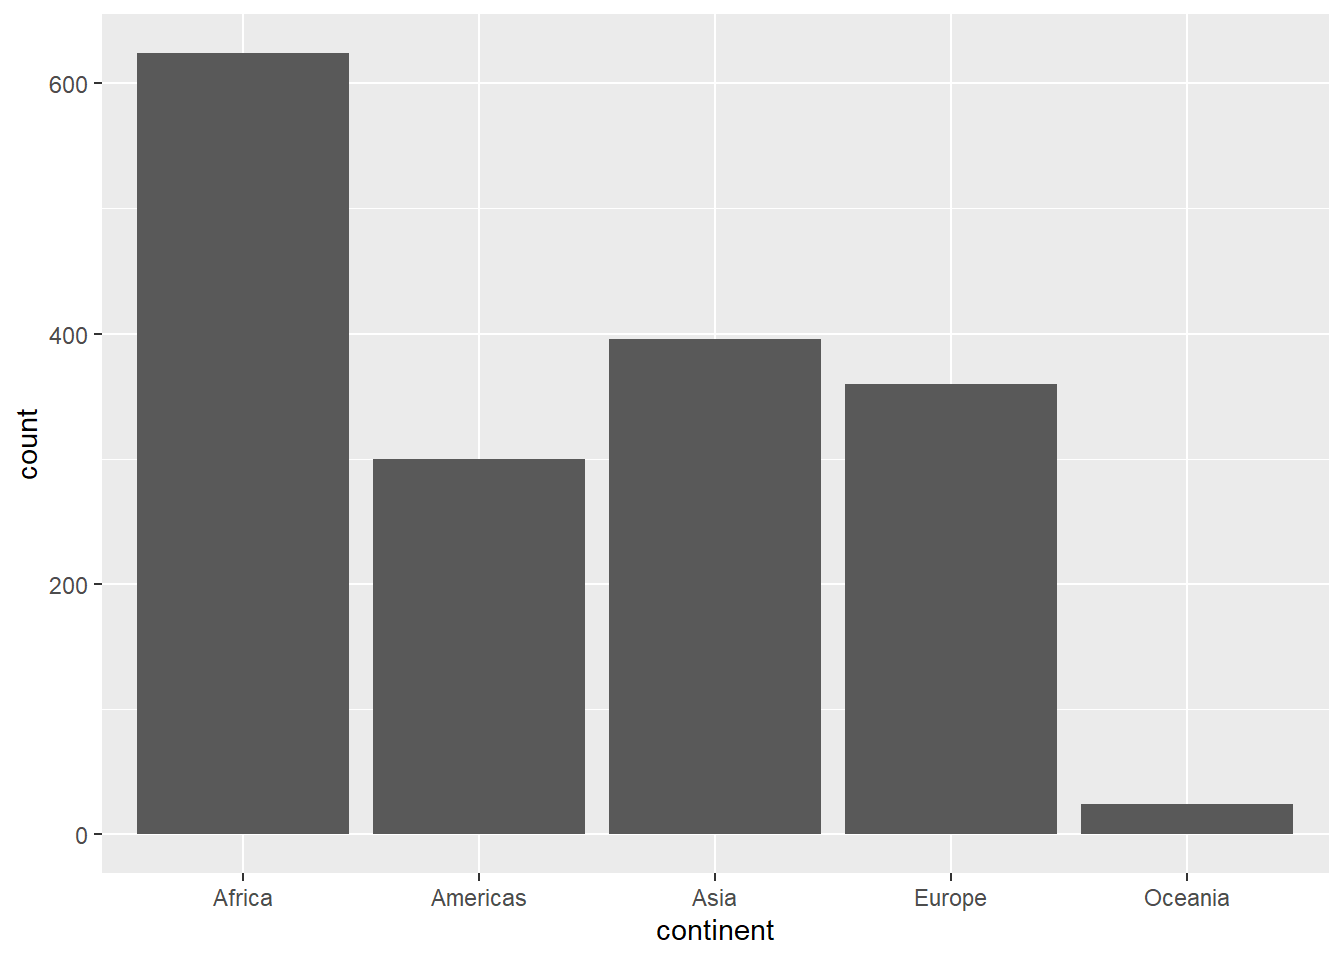
\includegraphics{Unsupervised-Learning_files/figure-latex/unnamed-chunk-4-1.pdf}

As it is clear, the distribution of the number of items is skewed to right, clearly most transactions inlcude fewer number of items, only very few have more than 10 items purchased together.

\hypertarget{support-count-item-frequencies-and-item-frequency-plot}{%
\section{Support Count (Item Frequencies) and Item Frequency Plot}\label{support-count-item-frequencies-and-item-frequency-plot}}

We can check the support count (\(freq(A)\)) for the top 25 products with the following R code:

\begin{Shaded}
\begin{Highlighting}[]
\NormalTok{itemSupportCount =}\StringTok{ }\KeywordTok{itemFrequency}\NormalTok{(Groceries, }\DataTypeTok{type =} \StringTok{"absolute"}\NormalTok{) }\CommentTok{# obtain the counts for individual items}
\NormalTok{itemSupportCount =}\StringTok{ }\KeywordTok{sort}\NormalTok{(itemSupportCount, }\DataTypeTok{decreasing =} \OtherTok{TRUE}\NormalTok{) }\CommentTok{# sort the counts in descending order}
\KeywordTok{head}\NormalTok{(itemSupportCount, }\DecValTok{25}\NormalTok{) }\CommentTok{# check the support count for the top 25 items}
\end{Highlighting}
\end{Shaded}

\begin{verbatim}
##            whole milk      other vegetables            rolls/buns 
##                  2513                  1903                  1809 
##                  soda                yogurt         bottled water 
##                  1715                  1372                  1087 
##       root vegetables        tropical fruit         shopping bags 
##                  1072                  1032                   969 
##               sausage                pastry          citrus fruit 
##                   924                   875                   814 
##          bottled beer            newspapers           canned beer 
##                   792                   785                   764 
##             pip fruit fruit/vegetable juice    whipped/sour cream 
##                   744                   711                   705 
##           brown bread         domestic eggs           frankfurter 
##                   638                   624                   580 
##             margarine                coffee                  pork 
##                   576                   571                   567 
##                butter 
##                   545
\end{verbatim}

We can also plot the support count, it is possible to change the colours of the bars as well.

\begin{Shaded}
\begin{Highlighting}[]
\KeywordTok{itemFrequencyPlot}\NormalTok{(Groceries, }\DataTypeTok{topN =} \DecValTok{25}\NormalTok{, }\DataTypeTok{type=}\StringTok{"absolute"}\NormalTok{)}
\end{Highlighting}
\end{Shaded}

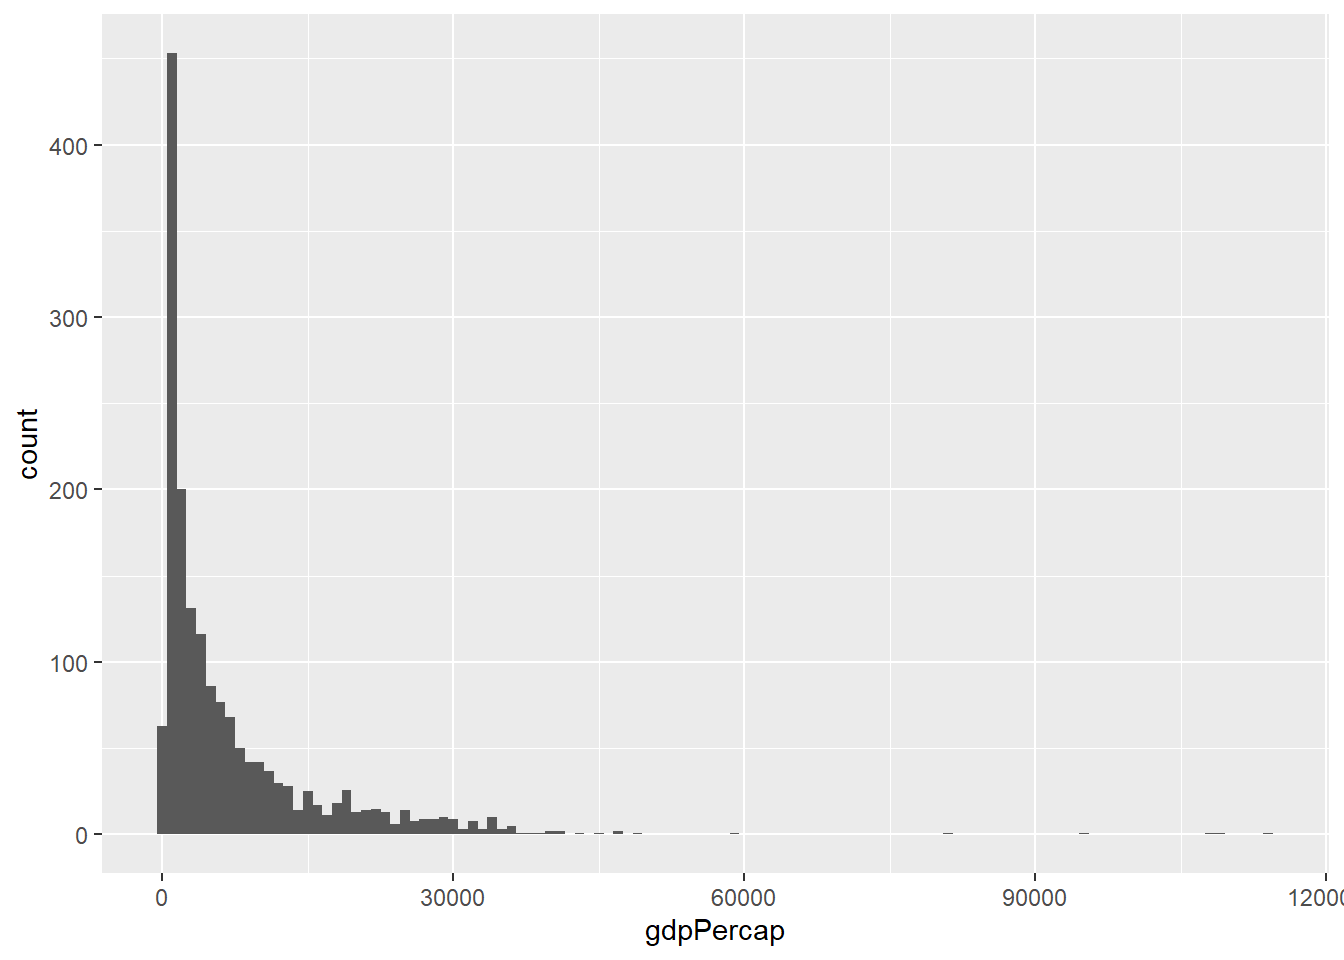
\includegraphics{Unsupervised-Learning_files/figure-latex/unnamed-chunk-6-1.pdf}

We can see that top purchased product is \{whole milk\} and it appears in 2513 transactions out of 9835. Therefore the support count for \{whole milk\} is 2513.

\hypertarget{support}{%
\section{Support}\label{support}}

Remember the support (\(S(A)\)) is calculated as follows:

\[S(A)=\frac{\texttt{freq({A})}}{n}\]
The support for \{whole milk\} would be

\[S(\texttt{{whole milk}})=\frac{\texttt{freq({whole milk})}}{n}=\frac{2513}{9835}=25.55\%\]

It is possible to obtain this information with the same code as shown previously by simply replacing \(\texttt{type="absolute"}\) with the \(\texttt{type="relative"}\) option:

\begin{Shaded}
\begin{Highlighting}[]
\NormalTok{itemSupport =}\StringTok{ }\KeywordTok{itemFrequency}\NormalTok{(Groceries, }\DataTypeTok{type =} \StringTok{"relative"}\NormalTok{) }\CommentTok{# obtain the counts for individual items}
\NormalTok{itemSupport =}\StringTok{ }\KeywordTok{sort}\NormalTok{(itemSupport, }\DataTypeTok{decreasing =} \OtherTok{TRUE}\NormalTok{) }\CommentTok{# sort the counts in descending order}
\KeywordTok{head}\NormalTok{(itemSupport, }\DecValTok{25}\NormalTok{) }\CommentTok{# check the support count for the top 25 items}
\end{Highlighting}
\end{Shaded}

\begin{verbatim}
##            whole milk      other vegetables            rolls/buns 
##            0.25551601            0.19349263            0.18393493 
##                  soda                yogurt         bottled water 
##            0.17437722            0.13950178            0.11052364 
##       root vegetables        tropical fruit         shopping bags 
##            0.10899847            0.10493137            0.09852567 
##               sausage                pastry          citrus fruit 
##            0.09395018            0.08896797            0.08276563 
##          bottled beer            newspapers           canned beer 
##            0.08052872            0.07981698            0.07768175 
##             pip fruit fruit/vegetable juice    whipped/sour cream 
##            0.07564820            0.07229283            0.07168277 
##           brown bread         domestic eggs           frankfurter 
##            0.06487036            0.06344687            0.05897306 
##             margarine                coffee                  pork 
##            0.05856634            0.05805796            0.05765125 
##                butter 
##            0.05541434
\end{verbatim}

We can also plot the support.

\begin{Shaded}
\begin{Highlighting}[]
\KeywordTok{itemFrequencyPlot}\NormalTok{(Groceries, }\DataTypeTok{topN =} \DecValTok{25}\NormalTok{, }\DataTypeTok{type=}\StringTok{"relative"}\NormalTok{)}
\end{Highlighting}
\end{Shaded}

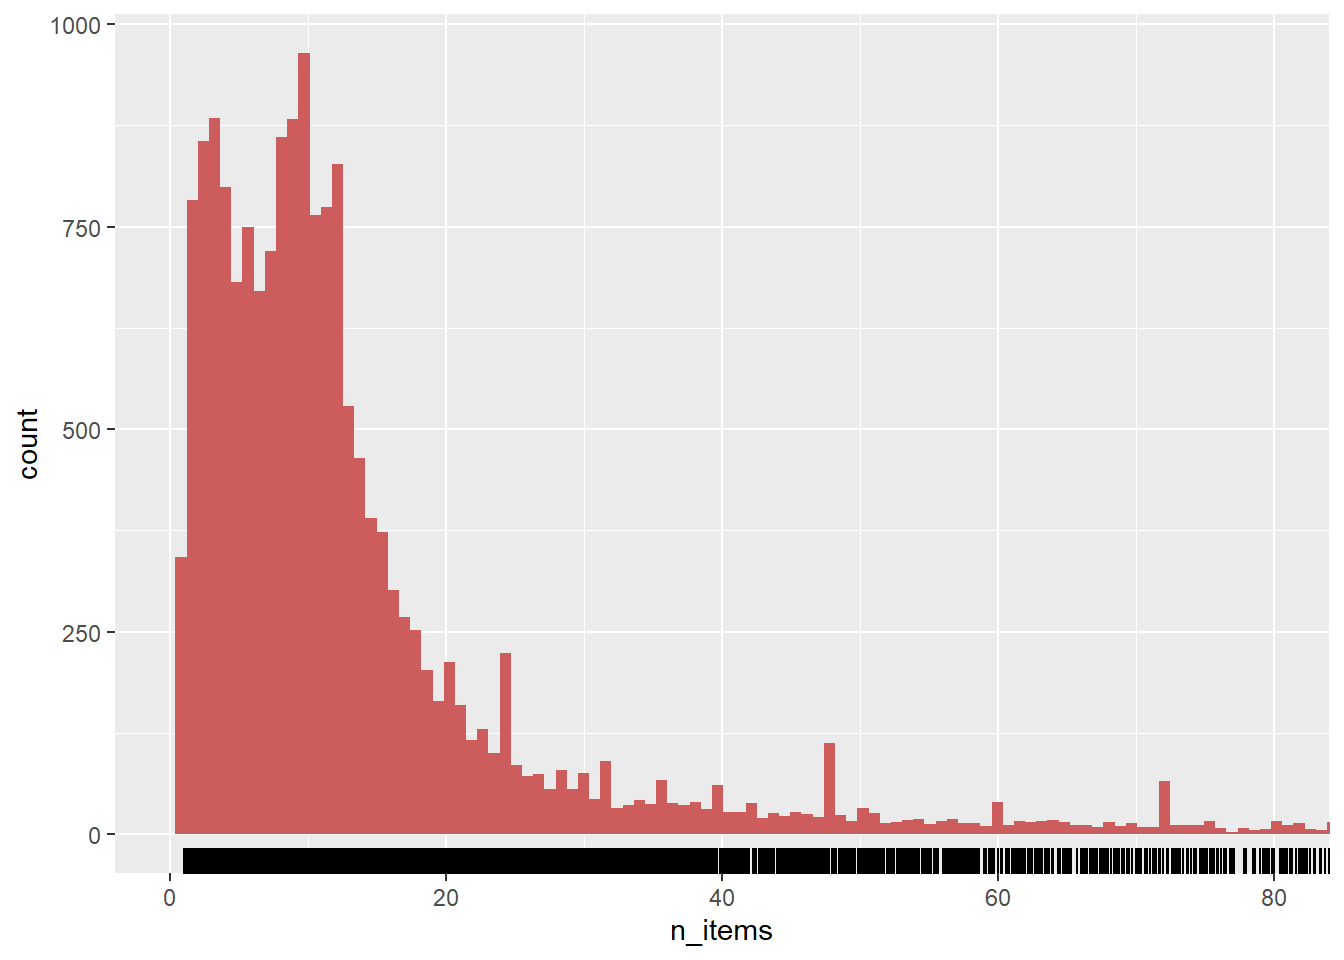
\includegraphics{Unsupervised-Learning_files/figure-latex/unnamed-chunk-8-1.pdf}

Note that the maximum support is low. To ensure that the top 25 frequent items are included in the analysis the minimum support would have to be less than 0.10! (\(10\%\)) Suppose we set the minimum support to 0.001 and minimum confidence to 0.8. We can mine some rules by executing the following R code:

\hypertarget{rule-generation-with-apriori-algorithm}{%
\section{Rule Generation with Apriori Algorithm}\label{rule-generation-with-apriori-algorithm}}

\begin{itemize}
\item
  We are going to use the Apriori algorithm within the \(\texttt{arules}\) library to mine frequent itemsets and association rules..
\item
  Assume that we want to generate all the rules that satisfy the support threshold of \(0.1\%\) and confidence threshold of \(80\%\), then we need to enter \(\texttt{supp=0.001}\) and \(\texttt{conf=0.8}\) values in the \(\texttt{apriori()}\) function. If you want stronger rules, you can increase the value of \(\texttt{conf}\) and for more extended rules give higher value to \(\texttt{maxlen}\).
\item
  It might be desirable to sort the rules according either confidence or support, here we chose sorting according to confidence in a descending manner.
\item
  Finally we can examine the rules using \(\texttt{summary()}\) function.
\end{itemize}

\begin{Shaded}
\begin{Highlighting}[]
\NormalTok{rules <-}\StringTok{ }\KeywordTok{apriori}\NormalTok{(Groceries, }\DataTypeTok{parameter =} \KeywordTok{list}\NormalTok{(}\DataTypeTok{supp=}\FloatTok{0.001}\NormalTok{, }\DataTypeTok{conf=}\FloatTok{0.8}\NormalTok{))}
\end{Highlighting}
\end{Shaded}

\begin{verbatim}
## Apriori
## 
## Parameter specification:
##  confidence minval smax arem  aval originalSupport maxtime support minlen
##         0.8    0.1    1 none FALSE            TRUE       5   0.001      1
##  maxlen target  ext
##      10  rules TRUE
## 
## Algorithmic control:
##  filter tree heap memopt load sort verbose
##     0.1 TRUE TRUE  FALSE TRUE    2    TRUE
## 
## Absolute minimum support count: 9 
## 
## set item appearances ...[0 item(s)] done [0.00s].
## set transactions ...[169 item(s), 9835 transaction(s)] done [0.01s].
## sorting and recoding items ... [157 item(s)] done [0.00s].
## creating transaction tree ... done [0.00s].
## checking subsets of size 1 2 3 4 5 6 done [0.04s].
## writing ... [410 rule(s)] done [0.06s].
## creating S4 object  ... done [0.00s].
\end{verbatim}

\begin{Shaded}
\begin{Highlighting}[]
\NormalTok{rules <-}\StringTok{ }\KeywordTok{sort}\NormalTok{(rules, }\DataTypeTok{by=}\StringTok{'confidence'}\NormalTok{, }\DataTypeTok{decreasing =} \OtherTok{TRUE}\NormalTok{)}
\KeywordTok{summary}\NormalTok{(rules)}
\end{Highlighting}
\end{Shaded}

\begin{verbatim}
## set of 410 rules
## 
## rule length distribution (lhs + rhs):sizes
##   3   4   5   6 
##  29 229 140  12 
## 
##    Min. 1st Qu.  Median    Mean 3rd Qu.    Max. 
##   3.000   4.000   4.000   4.329   5.000   6.000 
## 
## summary of quality measures:
##     support           confidence        coverage             lift       
##  Min.   :0.001017   Min.   :0.8000   Min.   :0.001017   Min.   : 3.131  
##  1st Qu.:0.001017   1st Qu.:0.8333   1st Qu.:0.001220   1st Qu.: 3.312  
##  Median :0.001220   Median :0.8462   Median :0.001322   Median : 3.588  
##  Mean   :0.001247   Mean   :0.8663   Mean   :0.001449   Mean   : 3.951  
##  3rd Qu.:0.001322   3rd Qu.:0.9091   3rd Qu.:0.001627   3rd Qu.: 4.341  
##  Max.   :0.003152   Max.   :1.0000   Max.   :0.003559   Max.   :11.235  
##      count      
##  Min.   :10.00  
##  1st Qu.:10.00  
##  Median :12.00  
##  Mean   :12.27  
##  3rd Qu.:13.00  
##  Max.   :31.00  
## 
## mining info:
##       data ntransactions support confidence
##  Groceries          9835   0.001        0.8
\end{verbatim}

In this output we are provided with the following information:

\begin{itemize}
\tightlist
\item
  There are 410 rules based on 0.001 support and 0.8 confidence thresholds.
\item
  The distribution of the number of items in each rule (rule length distribution): Most rules are 4 items long.
\end{itemize}

We need use the \(\texttt{inspect()}\) function to see the actual rules.

\begin{Shaded}
\begin{Highlighting}[]
\KeywordTok{inspect}\NormalTok{(rules[}\DecValTok{1}\OperatorTok{:}\DecValTok{5}\NormalTok{])}
\end{Highlighting}
\end{Shaded}

\begin{verbatim}
##     lhs                     rhs              support confidence    coverage     lift count
## [1] {rice,                                                                                
##      sugar}              => {whole milk} 0.001220132          1 0.001220132 3.913649    12
## [2] {canned fish,                                                                         
##      hygiene articles}   => {whole milk} 0.001118454          1 0.001118454 3.913649    11
## [3] {root vegetables,                                                                     
##      butter,                                                                              
##      rice}               => {whole milk} 0.001016777          1 0.001016777 3.913649    10
## [4] {root vegetables,                                                                     
##      whipped/sour cream,                                                                  
##      flour}              => {whole milk} 0.001728521          1 0.001728521 3.913649    17
## [5] {butter,                                                                              
##      soft cheese,                                                                         
##      domestic eggs}      => {whole milk} 0.001016777          1 0.001016777 3.913649    10
\end{verbatim}

If we look at the confidence we see that for the top 5 rules it is \(1\), this indicates \(100\%\) confidence:

\begin{itemize}
\item
  \(100\%\) customers who bought ``\{rice, sugar\}'' end up buying ``\{whole milk\}'' as well.
\item
  \(100\%\) customers who bought ``\{canned fish, hygiene articles\}'' end up buying ``\{whole milk\}'' as well.
\end{itemize}

In the following section we will look at visualizing the rules.

\hypertarget{visualisation-of-the-rules}{%
\subsection{Visualisation of the Rules}\label{visualisation-of-the-rules}}

\begin{Shaded}
\begin{Highlighting}[]
\NormalTok{topRules <-}\StringTok{ }\NormalTok{rules[}\DecValTok{1}\OperatorTok{:}\DecValTok{10}\NormalTok{]}
\KeywordTok{plot}\NormalTok{(topRules)}
\end{Highlighting}
\end{Shaded}

\begin{verbatim}
## To reduce overplotting, jitter is added! Use jitter = 0 to prevent jitter.
\end{verbatim}

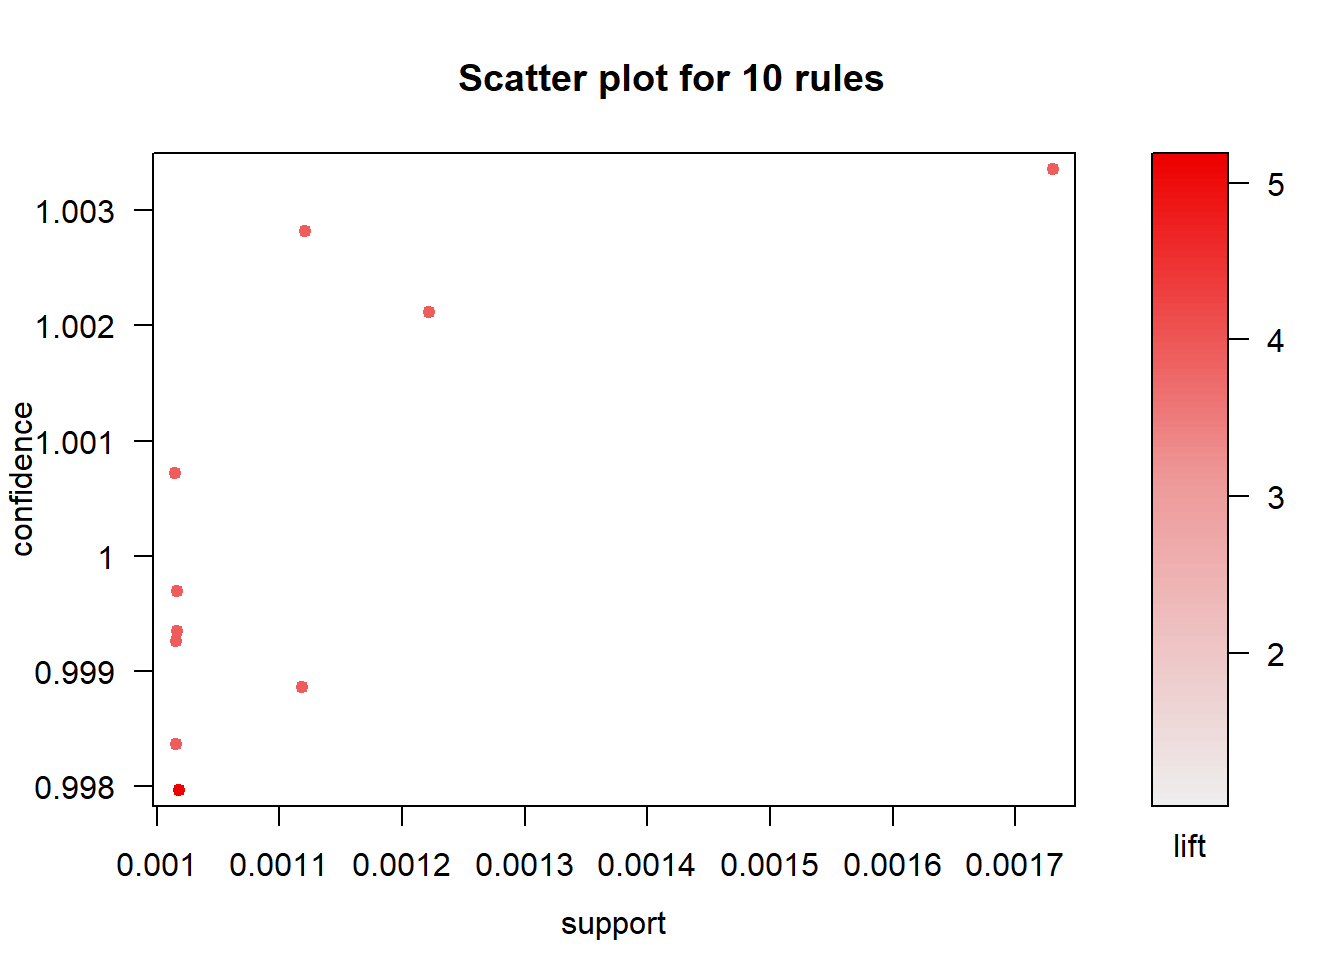
\includegraphics{Unsupervised-Learning_files/figure-latex/unnamed-chunk-11-1.pdf}

The scatter plot of support and confidence of the top ten rules shows us that high confidence rules have low support values.

\begin{Shaded}
\begin{Highlighting}[]
\KeywordTok{plot}\NormalTok{(rules)}
\end{Highlighting}
\end{Shaded}

\begin{verbatim}
## To reduce overplotting, jitter is added! Use jitter = 0 to prevent jitter.
\end{verbatim}

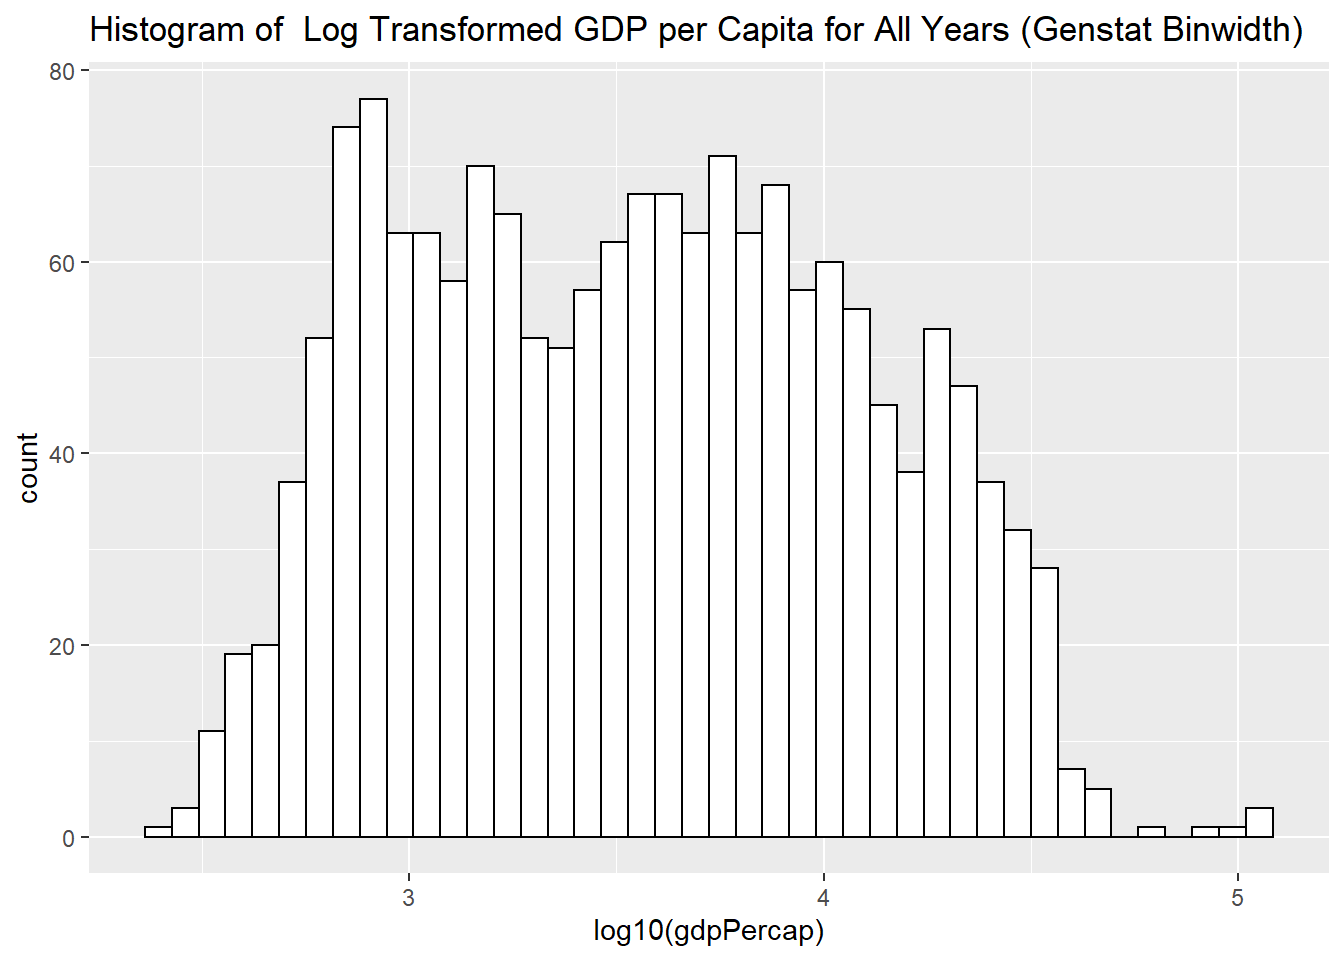
\includegraphics{Unsupervised-Learning_files/figure-latex/unnamed-chunk-12-1.pdf}

In the following section we will look at removing redundant rules.

\hypertarget{removing-redundant-rules}{%
\subsection{Removing redundant rules}\label{removing-redundant-rules}}

You may want to remove rules that are subsets of larger rules. Use the code below to remove such rules:

\begin{Shaded}
\begin{Highlighting}[]
\NormalTok{subset.rules <-}\StringTok{ }\KeywordTok{which}\NormalTok{(}\KeywordTok{colSums}\NormalTok{(}\KeywordTok{is.subset}\NormalTok{(rules, rules)) }\OperatorTok{>}\StringTok{ }\DecValTok{1}\NormalTok{) }\CommentTok{# get subset rules in vector}
\CommentTok{# is.subset() determines if elements of one vector contain all the elements of other}
\KeywordTok{length}\NormalTok{(subset.rules)}
\end{Highlighting}
\end{Shaded}

\begin{verbatim}
## [1] 91
\end{verbatim}

\begin{Shaded}
\begin{Highlighting}[]
\NormalTok{subset.rules <-}\StringTok{ }\NormalTok{rules[}\OperatorTok{-}\NormalTok{subset.rules] }\CommentTok{# remove subset rules.}
\end{Highlighting}
\end{Shaded}

\hypertarget{finding-rules-related-to-given-items}{%
\subsection{Finding rules related to given items}\label{finding-rules-related-to-given-items}}

In the case of specific product in interest, either as a precedent (LHS) or as a consequent (RHS) in the rule, you need to set the ``\(\texttt{appearance=}\)'' parameter in the apriori rule generating function:

Let us say we are interested in those transactions that end up in buying ``root vegetables'':

\begin{Shaded}
\begin{Highlighting}[]
\NormalTok{rveg.rules <-}\StringTok{ }\KeywordTok{apriori}\NormalTok{(Groceries, }\DataTypeTok{parameter =} \KeywordTok{list}\NormalTok{(}\DataTypeTok{supp=}\FloatTok{0.001}\NormalTok{, }\DataTypeTok{conf=}\FloatTok{0.8}\NormalTok{),}\DataTypeTok{appearance =} \KeywordTok{list}\NormalTok{(}\DataTypeTok{default=}\StringTok{"lhs"}\NormalTok{,}\DataTypeTok{rhs=}\StringTok{"root vegetables"}\NormalTok{))}
\end{Highlighting}
\end{Shaded}

\begin{verbatim}
## Apriori
## 
## Parameter specification:
##  confidence minval smax arem  aval originalSupport maxtime support minlen
##         0.8    0.1    1 none FALSE            TRUE       5   0.001      1
##  maxlen target  ext
##      10  rules TRUE
## 
## Algorithmic control:
##  filter tree heap memopt load sort verbose
##     0.1 TRUE TRUE  FALSE TRUE    2    TRUE
## 
## Absolute minimum support count: 9 
## 
## set item appearances ...[1 item(s)] done [0.00s].
## set transactions ...[169 item(s), 9835 transaction(s)] done [0.00s].
## sorting and recoding items ... [157 item(s)] done [0.00s].
## creating transaction tree ... done [0.00s].
## checking subsets of size 1 2 3 4 5 6 done [0.02s].
## writing ... [5 rule(s)] done [0.00s].
## creating S4 object  ... done [0.00s].
\end{verbatim}

\begin{Shaded}
\begin{Highlighting}[]
\KeywordTok{inspect}\NormalTok{(}\KeywordTok{head}\NormalTok{(rveg.rules))}
\end{Highlighting}
\end{Shaded}

\begin{verbatim}
##     lhs                        rhs                   support confidence    coverage     lift count
## [1] {other vegetables,                                                                            
##      whole milk,                                                                                  
##      yogurt,                                                                                      
##      rice}                  => {root vegetables} 0.001321810  0.8666667 0.001525165 7.951182    13
## [2] {tropical fruit,                                                                              
##      other vegetables,                                                                            
##      whole milk,                                                                                  
##      oil}                   => {root vegetables} 0.001321810  0.8666667 0.001525165 7.951182    13
## [3] {beef,                                                                                        
##      citrus fruit,                                                                                
##      tropical fruit,                                                                              
##      other vegetables}      => {root vegetables} 0.001016777  0.8333333 0.001220132 7.645367    10
## [4] {citrus fruit,                                                                                
##      other vegetables,                                                                            
##      soda,                                                                                        
##      fruit/vegetable juice} => {root vegetables} 0.001016777  0.9090909 0.001118454 8.340400    10
## [5] {tropical fruit,                                                                              
##      other vegetables,                                                                            
##      whole milk,                                                                                  
##      yogurt,                                                                                      
##      oil}                   => {root vegetables} 0.001016777  0.9090909 0.001118454 8.340400    10
\end{verbatim}

\hypertarget{using-your-own-dataset-stored-as-a-csv-file}{%
\section{Using your own dataset stored as a csv file}\label{using-your-own-dataset-stored-as-a-csv-file}}

You might want to use a dataset from a csv file. The format of this file should be as follows:

\begin{itemize}
\tightlist
\item
  Transactions in the rows (remember in our small example, we had 5 transactions.)
\item
  Items per transaction should be entered separately in different columns (items were A, B, C, D, E, and F)
\end{itemize}

\begin{figure}
\centering
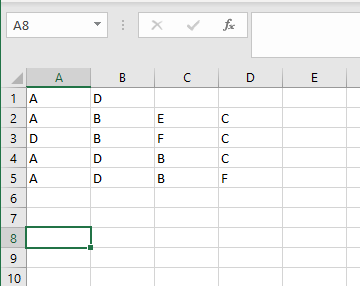
\includegraphics{example.png}
\caption{How the data looks like in csv format:}
\end{figure}

\begin{itemize}
\tightlist
\item
  The data should be extracted using the \(\texttt{read.transactions()}\) function.
\end{itemize}

\begin{Shaded}
\begin{Highlighting}[]
\NormalTok{slideExample <-}\StringTok{ }\KeywordTok{read.transactions}\NormalTok{(}\StringTok{'C:/Users/01438475/Google Drive/UCTcourses/Analytics/UnsupervisedLearning/Arules/example.csv'}\NormalTok{, }\DataTypeTok{format =} \StringTok{'basket'}\NormalTok{, }\DataTypeTok{sep=}\StringTok{','}\NormalTok{)}
\NormalTok{slideExample}
\end{Highlighting}
\end{Shaded}

\begin{verbatim}
## transactions in sparse format with
##  5 transactions (rows) and
##  6 items (columns)
\end{verbatim}

\begin{Shaded}
\begin{Highlighting}[]
\KeywordTok{inspect}\NormalTok{(}\KeywordTok{head}\NormalTok{(slideExample, }\DecValTok{6}\NormalTok{))}
\end{Highlighting}
\end{Shaded}

\begin{verbatim}
##     items    
## [1] {A,D}    
## [2] {A,B,C,E}
## [3] {B,C,D,F}
## [4] {A,B,C,D}
## [5] {A,B,D,F}
\end{verbatim}

\begin{Shaded}
\begin{Highlighting}[]
\KeywordTok{size}\NormalTok{(}\KeywordTok{head}\NormalTok{(slideExample))}
\end{Highlighting}
\end{Shaded}

\begin{verbatim}
## [1] 2 4 4 4 4
\end{verbatim}

I will leave all the rest for you to obtain.

\hypertarget{references}{%
\section{References:}\label{references}}

\begin{itemize}
\tightlist
\item
  \href{http://www.rdatamining.com/examples/association-rules}{R and Data Mining}
\item
  \href{https://github.com/susanli2016/Data-Analysis-with-R/blob/master/Market_Basket_Analysis.Rmd}{Susan Li - MBA}
\item
  \href{https://www.datacamp.com/community/tutorials/market-basket-analysis-r}{Datacamp}
\item
  Dr Juwa Nyirenda's lecture notes
\end{itemize}

\hypertarget{cluster-analysis}{%
\chapter{Cluster Analysis}\label{cluster-analysis}}

We will use the built-in R dataset USArrest which contains statistics, in arrests per 100,000 residents for assault, murder, and rape in each of the 50 US states in 1973. It includes also the percent of the population living in urban areas. It contains 50 observations on 4 variables:

\hypertarget{prerequisites}{%
\section{Prerequisites}\label{prerequisites}}

We will need the following packages:

\begin{Shaded}
\begin{Highlighting}[]
\KeywordTok{library}\NormalTok{(cluster)}
\KeywordTok{library}\NormalTok{(NbClust)}
\KeywordTok{library}\NormalTok{(fpc)}
\end{Highlighting}
\end{Shaded}

Load the data set

\begin{Shaded}
\begin{Highlighting}[]
\KeywordTok{data}\NormalTok{(}\StringTok{"USArrests"}\NormalTok{)}
\CommentTok{# Remove any missing value (i.e, NA values for not available)}
\CommentTok{# That might be present in the data}
\NormalTok{df <-}\StringTok{ }\KeywordTok{na.omit}\NormalTok{(USArrests)}
\CommentTok{# View the firt 6 rows of the data}
\KeywordTok{head}\NormalTok{(df, }\DataTypeTok{n =} \DecValTok{6}\NormalTok{)}
\end{Highlighting}
\end{Shaded}

\begin{verbatim}
##            Murder Assault UrbanPop Rape
## Alabama      13.2     236       58 21.2
## Alaska       10.0     263       48 44.5
## Arizona       8.1     294       80 31.0
## Arkansas      8.8     190       50 19.5
## California    9.0     276       91 40.6
## Colorado      7.9     204       78 38.7
\end{verbatim}

Before clustering is done, we can compute some descriptive statistics for the data

\begin{Shaded}
\begin{Highlighting}[]
\NormalTok{desc_stats <-}\StringTok{ }\KeywordTok{data.frame}\NormalTok{(}
\DataTypeTok{Min =} \KeywordTok{apply}\NormalTok{(df, }\DecValTok{2}\NormalTok{, min), }\CommentTok{# minimum}
\DataTypeTok{Med =} \KeywordTok{apply}\NormalTok{(df, }\DecValTok{2}\NormalTok{, median), }\CommentTok{# median}
\DataTypeTok{Mean =} \KeywordTok{apply}\NormalTok{(df, }\DecValTok{2}\NormalTok{, mean), }\CommentTok{# mean}
\DataTypeTok{SD =} \KeywordTok{apply}\NormalTok{(df, }\DecValTok{2}\NormalTok{, sd), }\CommentTok{# Standard deviation}
\DataTypeTok{Max =} \KeywordTok{apply}\NormalTok{(df, }\DecValTok{2}\NormalTok{, max) }\CommentTok{# Maximum}
\NormalTok{)}
\NormalTok{desc_stats <-}\StringTok{ }\KeywordTok{round}\NormalTok{(desc_stats, }\DecValTok{1}\NormalTok{)}
\KeywordTok{head}\NormalTok{(desc_stats)}
\end{Highlighting}
\end{Shaded}

\begin{verbatim}
##           Min   Med  Mean   SD   Max
## Murder    0.8   7.2   7.8  4.4  17.4
## Assault  45.0 159.0 170.8 83.3 337.0
## UrbanPop 32.0  66.0  65.5 14.5  91.0
## Rape      7.3  20.1  21.2  9.4  46.0
\end{verbatim}

Note that the variables have large different means and variances. Therfore we need to standardise them.

\begin{Shaded}
\begin{Highlighting}[]
\NormalTok{df <-}\StringTok{ }\KeywordTok{scale}\NormalTok{(df)}
\KeywordTok{head}\NormalTok{(df)}
\end{Highlighting}
\end{Shaded}

\begin{verbatim}
##                Murder   Assault   UrbanPop         Rape
## Alabama    1.24256408 0.7828393 -0.5209066 -0.003416473
## Alaska     0.50786248 1.1068225 -1.2117642  2.484202941
## Arizona    0.07163341 1.4788032  0.9989801  1.042878388
## Arkansas   0.23234938 0.2308680 -1.0735927 -0.184916602
## California 0.27826823 1.2628144  1.7589234  2.067820292
## Colorado   0.02571456 0.3988593  0.8608085  1.864967207
\end{verbatim}

For partition clustering methods we will assume that K=2 clusters

\hypertarget{k-means-clustering}{%
\section{K-means clustering}\label{k-means-clustering}}

We will use the kmeans() function in the stats package.

\begin{Shaded}
\begin{Highlighting}[]
\KeywordTok{set.seed}\NormalTok{(}\DecValTok{123}\NormalTok{)}
\NormalTok{km.out <-}\StringTok{ }\KeywordTok{kmeans}\NormalTok{(df, }\DecValTok{2}\NormalTok{, }\DataTypeTok{nstart =} \DecValTok{25}\NormalTok{)}
\CommentTok{# k-means group number of each observation}
\NormalTok{km.out}\OperatorTok{$}\NormalTok{cluster}
\end{Highlighting}
\end{Shaded}

\begin{verbatim}
##        Alabama         Alaska        Arizona       Arkansas     California 
##              1              1              1              2              1 
##       Colorado    Connecticut       Delaware        Florida        Georgia 
##              1              2              2              1              1 
##         Hawaii          Idaho       Illinois        Indiana           Iowa 
##              2              2              1              2              2 
##         Kansas       Kentucky      Louisiana          Maine       Maryland 
##              2              2              1              2              1 
##  Massachusetts       Michigan      Minnesota    Mississippi       Missouri 
##              2              1              2              1              1 
##        Montana       Nebraska         Nevada  New Hampshire     New Jersey 
##              2              2              1              2              2 
##     New Mexico       New York North Carolina   North Dakota           Ohio 
##              1              1              1              2              2 
##       Oklahoma         Oregon   Pennsylvania   Rhode Island South Carolina 
##              2              2              2              2              1 
##   South Dakota      Tennessee          Texas           Utah        Vermont 
##              2              1              1              2              2 
##       Virginia     Washington  West Virginia      Wisconsin        Wyoming 
##              2              2              2              2              2
\end{verbatim}

\hypertarget{k-medoids-clustering}{%
\section{K-medoids clustering}\label{k-medoids-clustering}}

We will use the pam() in the cluster package.

\begin{Shaded}
\begin{Highlighting}[]
\NormalTok{pam.out <-}\StringTok{ }\KeywordTok{pam}\NormalTok{(df, }\DecValTok{2}\NormalTok{)}
\NormalTok{pam.out}\OperatorTok{$}\NormalTok{cluster}
\end{Highlighting}
\end{Shaded}

\begin{verbatim}
##        Alabama         Alaska        Arizona       Arkansas     California 
##              1              1              1              2              1 
##       Colorado    Connecticut       Delaware        Florida        Georgia 
##              1              2              2              1              1 
##         Hawaii          Idaho       Illinois        Indiana           Iowa 
##              2              2              1              2              2 
##         Kansas       Kentucky      Louisiana          Maine       Maryland 
##              2              2              1              2              1 
##  Massachusetts       Michigan      Minnesota    Mississippi       Missouri 
##              2              1              2              1              1 
##        Montana       Nebraska         Nevada  New Hampshire     New Jersey 
##              2              2              1              2              2 
##     New Mexico       New York North Carolina   North Dakota           Ohio 
##              1              1              1              2              2 
##       Oklahoma         Oregon   Pennsylvania   Rhode Island South Carolina 
##              2              2              2              2              1 
##   South Dakota      Tennessee          Texas           Utah        Vermont 
##              2              1              1              2              2 
##       Virginia     Washington  West Virginia      Wisconsin        Wyoming 
##              2              2              2              2              2
\end{verbatim}

\hypertarget{hierarchical-clustering}{%
\section{Hierarchical Clustering}\label{hierarchical-clustering}}

Here the built-in R function hclust() is used:

\hypertarget{compute-pairewise-distance-matrices}{%
\subsection{Compute pairewise distance matrices}\label{compute-pairewise-distance-matrices}}

\begin{Shaded}
\begin{Highlighting}[]
\NormalTok{dist.out <-}\StringTok{ }\KeywordTok{dist}\NormalTok{(df, }\DataTypeTok{method =} \StringTok{"euclidean"}\NormalTok{)}
\end{Highlighting}
\end{Shaded}

\hypertarget{single-linkage}{%
\subsection{Single Linkage}\label{single-linkage}}

\begin{Shaded}
\begin{Highlighting}[]
\NormalTok{out.single.euc <-}\StringTok{ }\KeywordTok{hclust}\NormalTok{(}\KeywordTok{daisy}\NormalTok{(df,}\DataTypeTok{metric=}\StringTok{"euclidean"}\NormalTok{),}\DataTypeTok{method=}\StringTok{"single"}\NormalTok{) }

\CommentTok{# try other metric="euclidean"}
\KeywordTok{plot}\NormalTok{(out.single.euc)}
\end{Highlighting}
\end{Shaded}

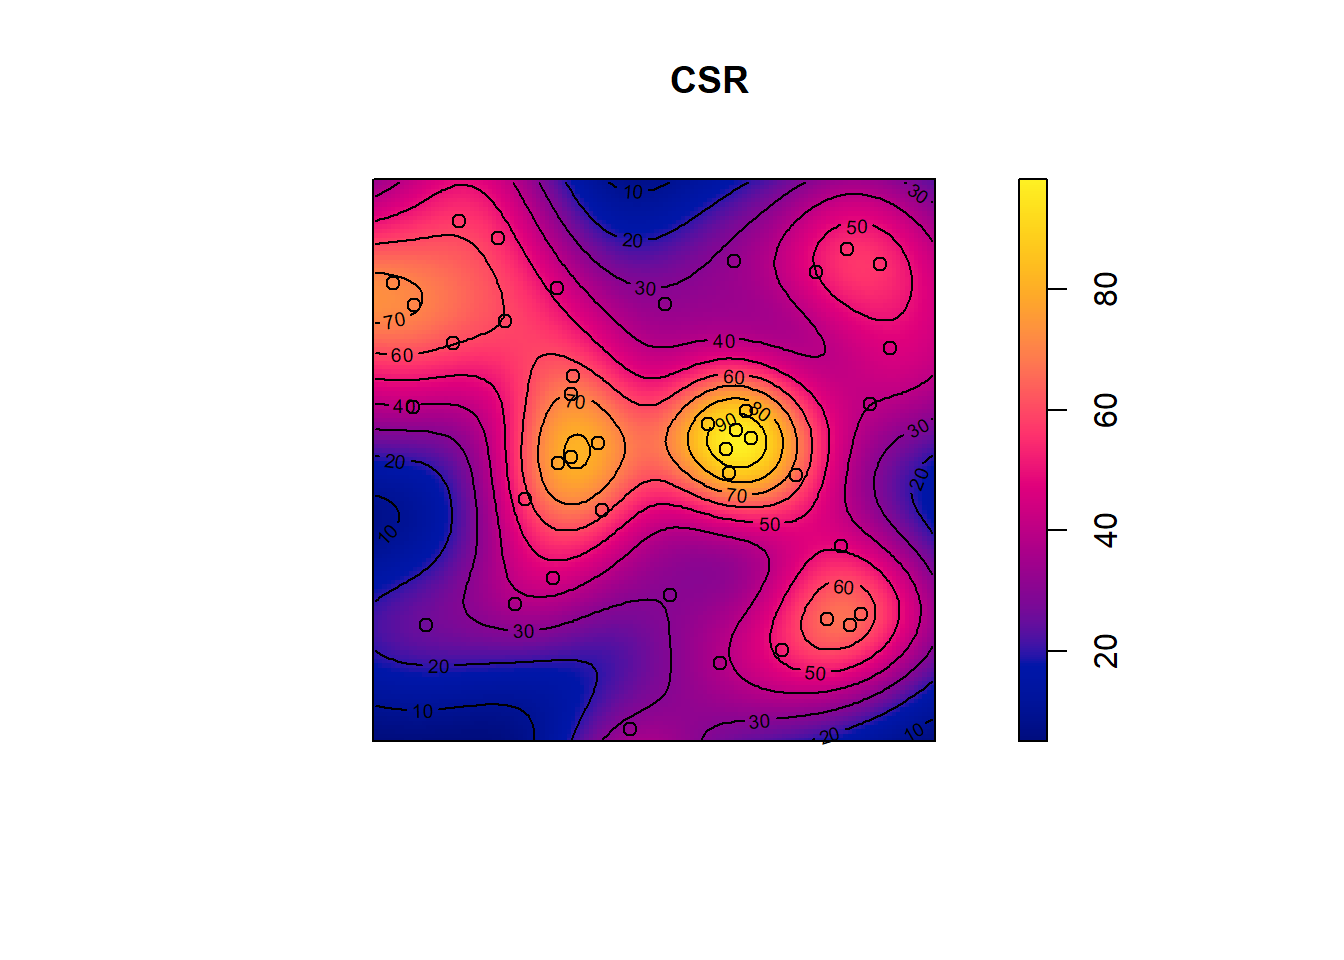
\includegraphics{Unsupervised-Learning_files/figure-latex/unnamed-chunk-23-1.pdf}

\begin{Shaded}
\begin{Highlighting}[]
 \CommentTok{# decide to cut the tree at height 1}
\NormalTok{out.single.euc <-}\StringTok{ }\KeywordTok{cutree}\NormalTok{(out.single.euc, }\DataTypeTok{h=}\FloatTok{1.5}\NormalTok{)}
 \CommentTok{# view cluster allocation}
\KeywordTok{names}\NormalTok{ (out.single.euc) <-}\StringTok{ }\KeywordTok{rownames}\NormalTok{(df)}
\KeywordTok{sort}\NormalTok{(out.single.euc)}
\end{Highlighting}
\end{Shaded}

\begin{verbatim}
##        Alabama        Arizona       Arkansas     California       Colorado 
##              1              1              1              1              1 
##    Connecticut       Delaware        Florida        Georgia         Hawaii 
##              1              1              1              1              1 
##          Idaho       Illinois        Indiana           Iowa         Kansas 
##              1              1              1              1              1 
##       Kentucky      Louisiana          Maine       Maryland  Massachusetts 
##              1              1              1              1              1 
##       Michigan      Minnesota    Mississippi       Missouri        Montana 
##              1              1              1              1              1 
##       Nebraska         Nevada  New Hampshire     New Jersey     New Mexico 
##              1              1              1              1              1 
##       New York North Carolina   North Dakota           Ohio       Oklahoma 
##              1              1              1              1              1 
##         Oregon   Pennsylvania   Rhode Island South Carolina   South Dakota 
##              1              1              1              1              1 
##      Tennessee          Texas           Utah        Vermont       Virginia 
##              1              1              1              1              1 
##     Washington  West Virginia      Wisconsin        Wyoming         Alaska 
##              1              1              1              1              2
\end{verbatim}

\hypertarget{complete-linkage}{%
\subsection{Complete Linkage}\label{complete-linkage}}

\begin{Shaded}
\begin{Highlighting}[]
\NormalTok{hc <-}\StringTok{ }\KeywordTok{hclust}\NormalTok{(dist.out, }\DataTypeTok{method =} \StringTok{"complete"}\NormalTok{)}
\end{Highlighting}
\end{Shaded}

Visualization of hclust

\begin{Shaded}
\begin{Highlighting}[]
\KeywordTok{plot}\NormalTok{(hc, }\DataTypeTok{labels =}\NormalTok{ F,}\OperatorTok{-}\DecValTok{1}\NormalTok{)}
\KeywordTok{rect.hclust}\NormalTok{(hc, }\DataTypeTok{k =} \DecValTok{2}\NormalTok{, }\DataTypeTok{border =} \DecValTok{2}\OperatorTok{:}\DecValTok{3}\NormalTok{) }\CommentTok{# Add rectangle around 2 clusters, try with 3?}
\end{Highlighting}
\end{Shaded}

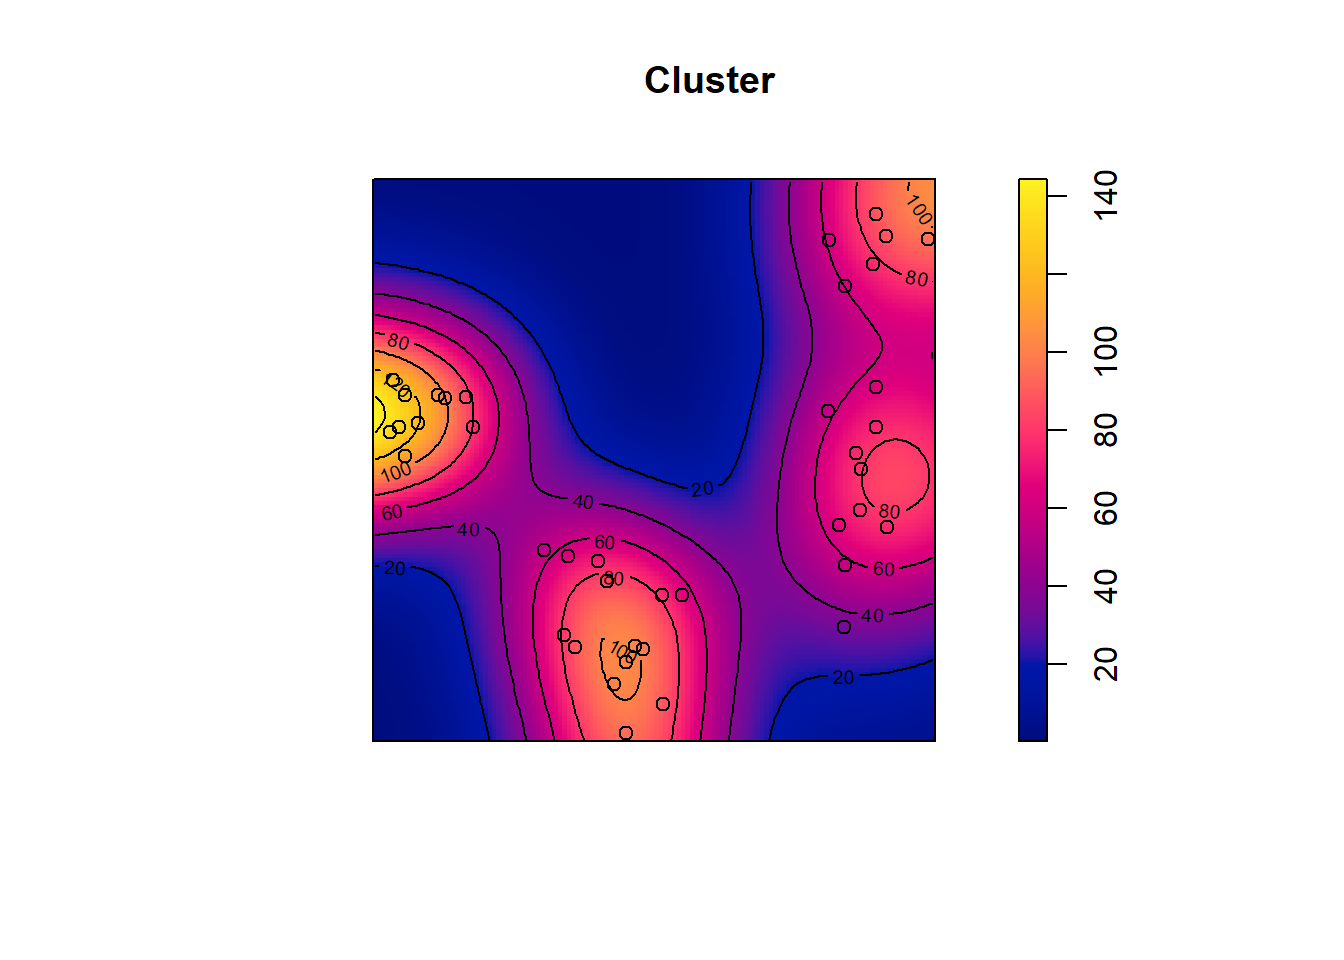
\includegraphics{Unsupervised-Learning_files/figure-latex/unnamed-chunk-25-1.pdf}

\hypertarget{centroid}{%
\subsection{Centroid}\label{centroid}}

\begin{Shaded}
\begin{Highlighting}[]
\CommentTok{# Centroid clustering}
\NormalTok{out.centroid.euc <-}\StringTok{ }\KeywordTok{hclust}\NormalTok{(}\KeywordTok{daisy}\NormalTok{(df,}\DataTypeTok{metric=}\StringTok{"euclidean"}\NormalTok{),}\DataTypeTok{method=}\StringTok{"centroid"}\NormalTok{)}
\KeywordTok{plot}\NormalTok{(out.centroid.euc)}
\end{Highlighting}
\end{Shaded}

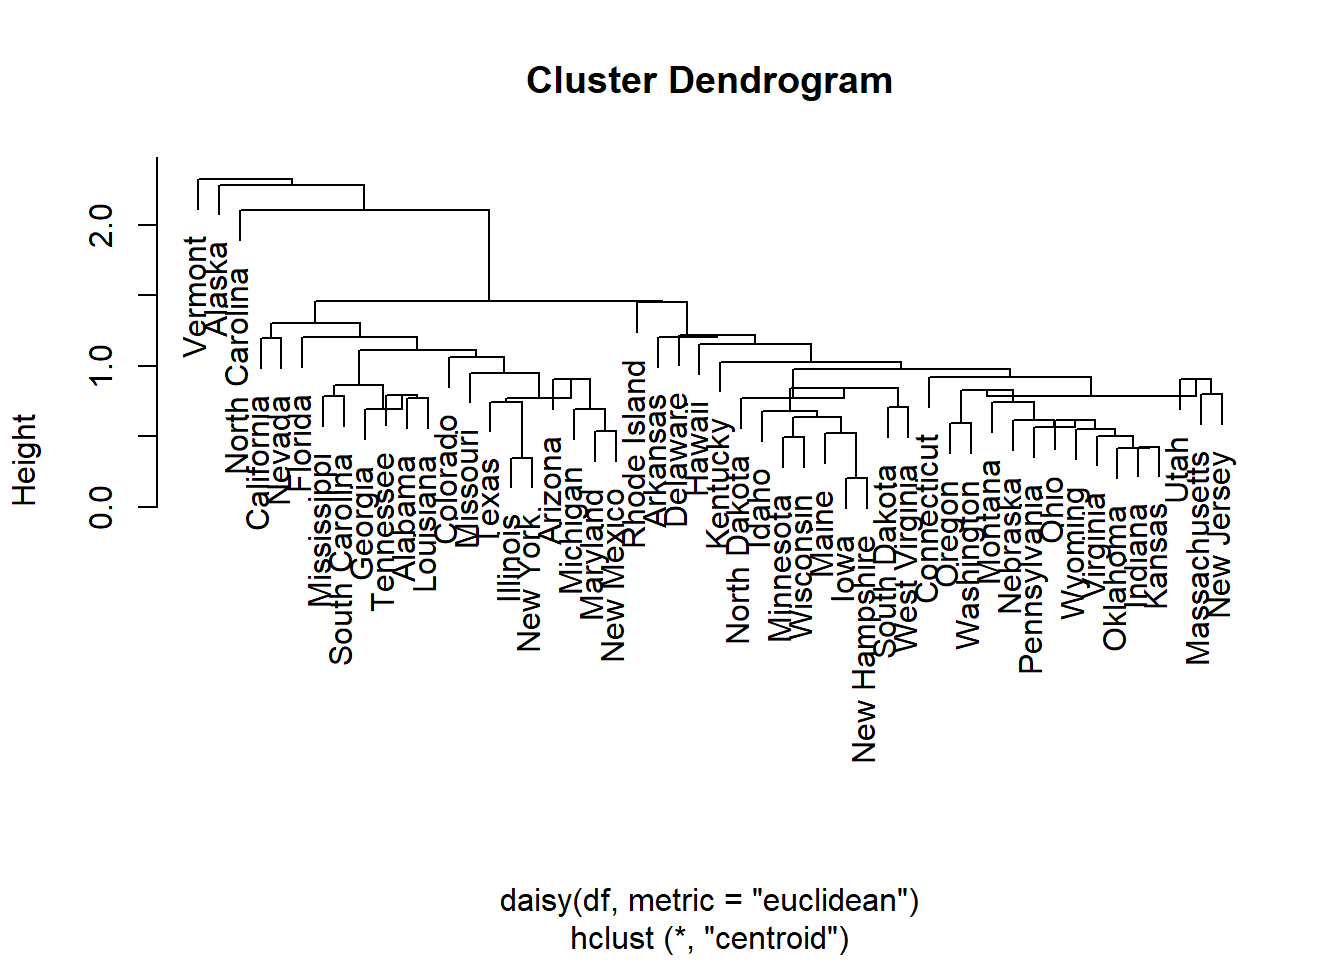
\includegraphics{Unsupervised-Learning_files/figure-latex/unnamed-chunk-26-1.pdf}

\begin{Shaded}
\begin{Highlighting}[]
\NormalTok{out.centroid.city <-}\StringTok{ }\KeywordTok{hclust}\NormalTok{(}\KeywordTok{daisy}\NormalTok{(df,}\DataTypeTok{metric=}\StringTok{"manhattan"}\NormalTok{),}\DataTypeTok{method=}\StringTok{"centroid"}\NormalTok{)}
\KeywordTok{plot}\NormalTok{(out.centroid.city)}
\end{Highlighting}
\end{Shaded}

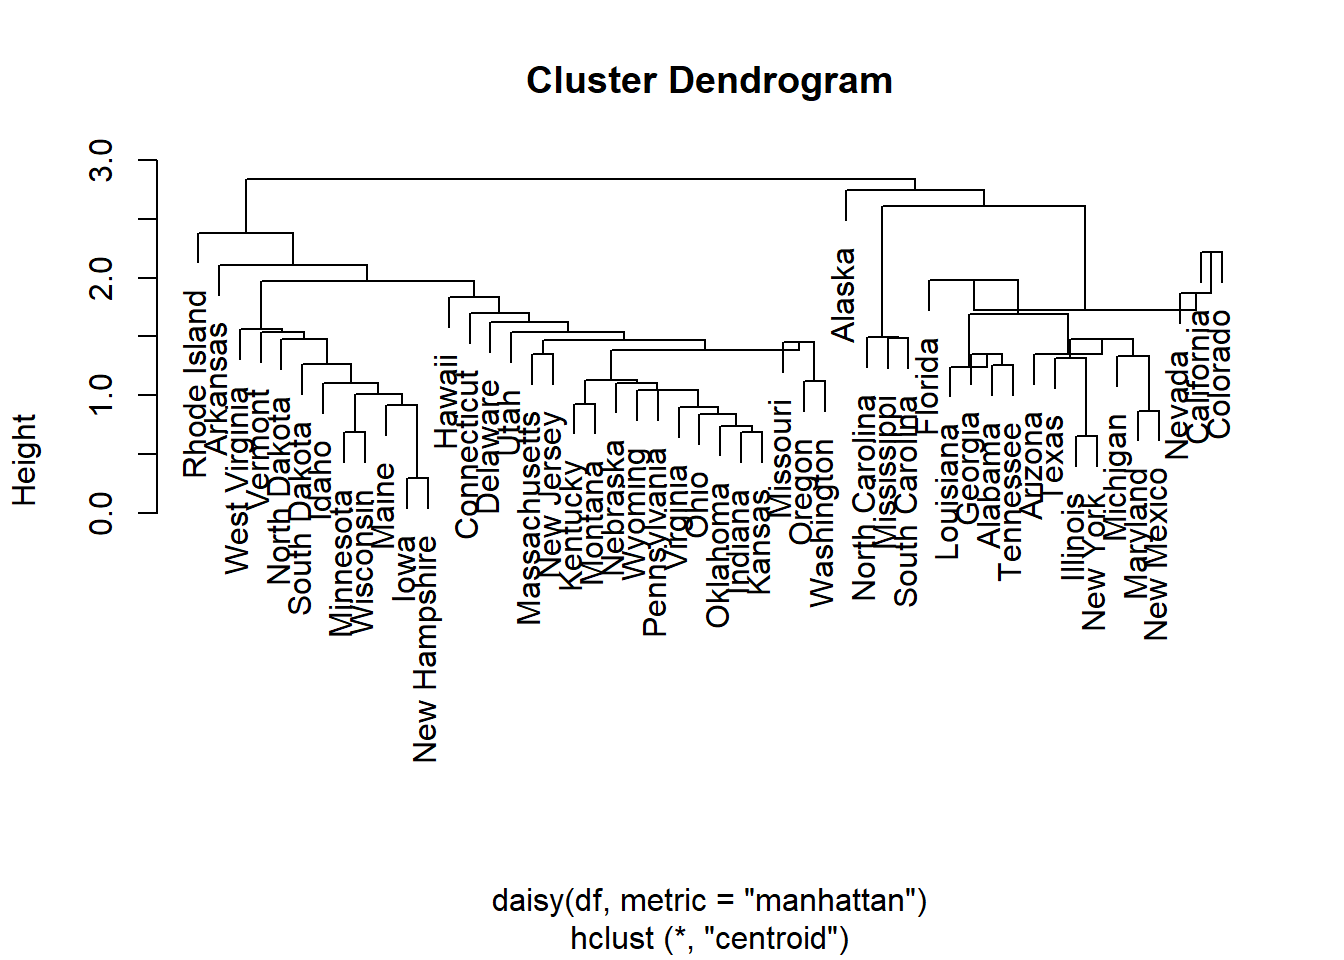
\includegraphics{Unsupervised-Learning_files/figure-latex/unnamed-chunk-26-2.pdf}

\begin{Shaded}
\begin{Highlighting}[]
\NormalTok{out.centroid.cor <-}\StringTok{ }\KeywordTok{hclust}\NormalTok{(}\KeywordTok{as.dist}\NormalTok{(}\DecValTok{1}\OperatorTok{-}\KeywordTok{cor}\NormalTok{(}\KeywordTok{t}\NormalTok{(df))),}\DataTypeTok{method=}\StringTok{"centroid"}\NormalTok{)}
\KeywordTok{plot}\NormalTok{(out.centroid.cor)}
\end{Highlighting}
\end{Shaded}

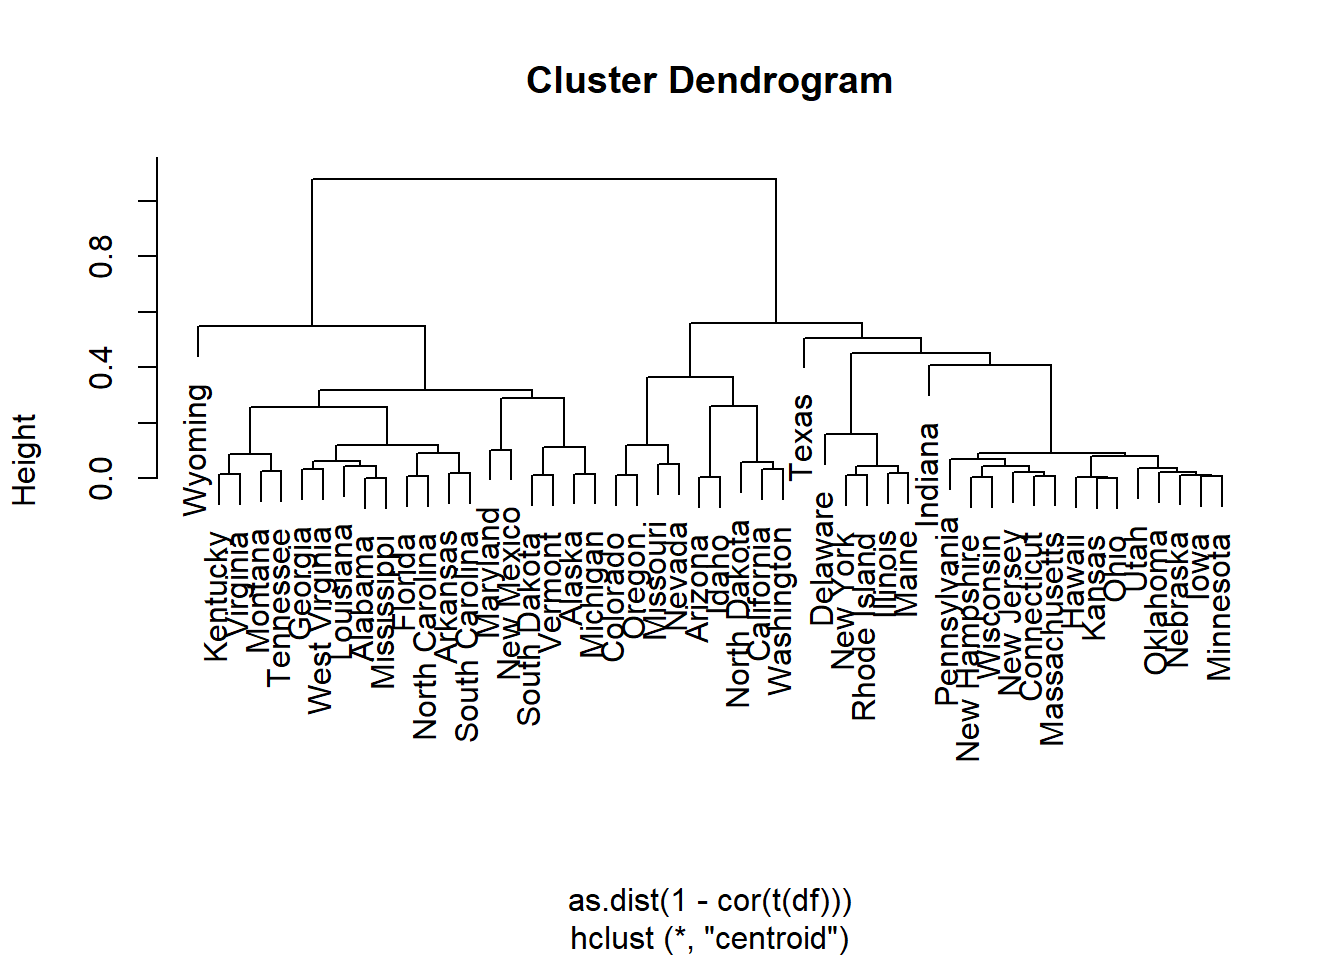
\includegraphics{Unsupervised-Learning_files/figure-latex/unnamed-chunk-26-3.pdf}

\hypertarget{methods-for-determining-number-of-clusters}{%
\section{Methods for determining number of clusters}\label{methods-for-determining-number-of-clusters}}

\hypertarget{elbow-method-for-k-means-clustering}{%
\subsection{Elbow method for k-means clustering}\label{elbow-method-for-k-means-clustering}}

\begin{Shaded}
\begin{Highlighting}[]
\KeywordTok{set.seed}\NormalTok{(}\DecValTok{123}\NormalTok{)}
\CommentTok{# Compute and plot wss for k = 2 to k = 15}
\NormalTok{k.max <-}\StringTok{ }\DecValTok{15} \CommentTok{# Maximal number of clusters}
\NormalTok{df.out <-}\StringTok{ }\NormalTok{df}
\NormalTok{wss <-}\StringTok{ }\KeywordTok{sapply}\NormalTok{(}\DecValTok{1}\OperatorTok{:}\NormalTok{k.max,}
\ControlFlowTok{function}\NormalTok{(k)\{}\KeywordTok{kmeans}\NormalTok{(df.out, k, }\DataTypeTok{nstart=}\DecValTok{10}\NormalTok{ )}\OperatorTok{$}\NormalTok{tot.withinss\})}
\KeywordTok{plot}\NormalTok{(}\DecValTok{1}\OperatorTok{:}\NormalTok{k.max, wss, }\DataTypeTok{type=}\StringTok{"b"}\NormalTok{, }\DataTypeTok{pch =} \DecValTok{19}\NormalTok{, }\DataTypeTok{frame =} \OtherTok{FALSE}\NormalTok{, }\DataTypeTok{xlab=}\StringTok{"Number of clusters K"}\NormalTok{, }\DataTypeTok{ylab=}\StringTok{"Total within-clusters sum of squares"}\NormalTok{)}
\KeywordTok{abline}\NormalTok{(}\DataTypeTok{v =} \DecValTok{3}\NormalTok{, }\DataTypeTok{lty =}\DecValTok{2}\NormalTok{)}
\end{Highlighting}
\end{Shaded}

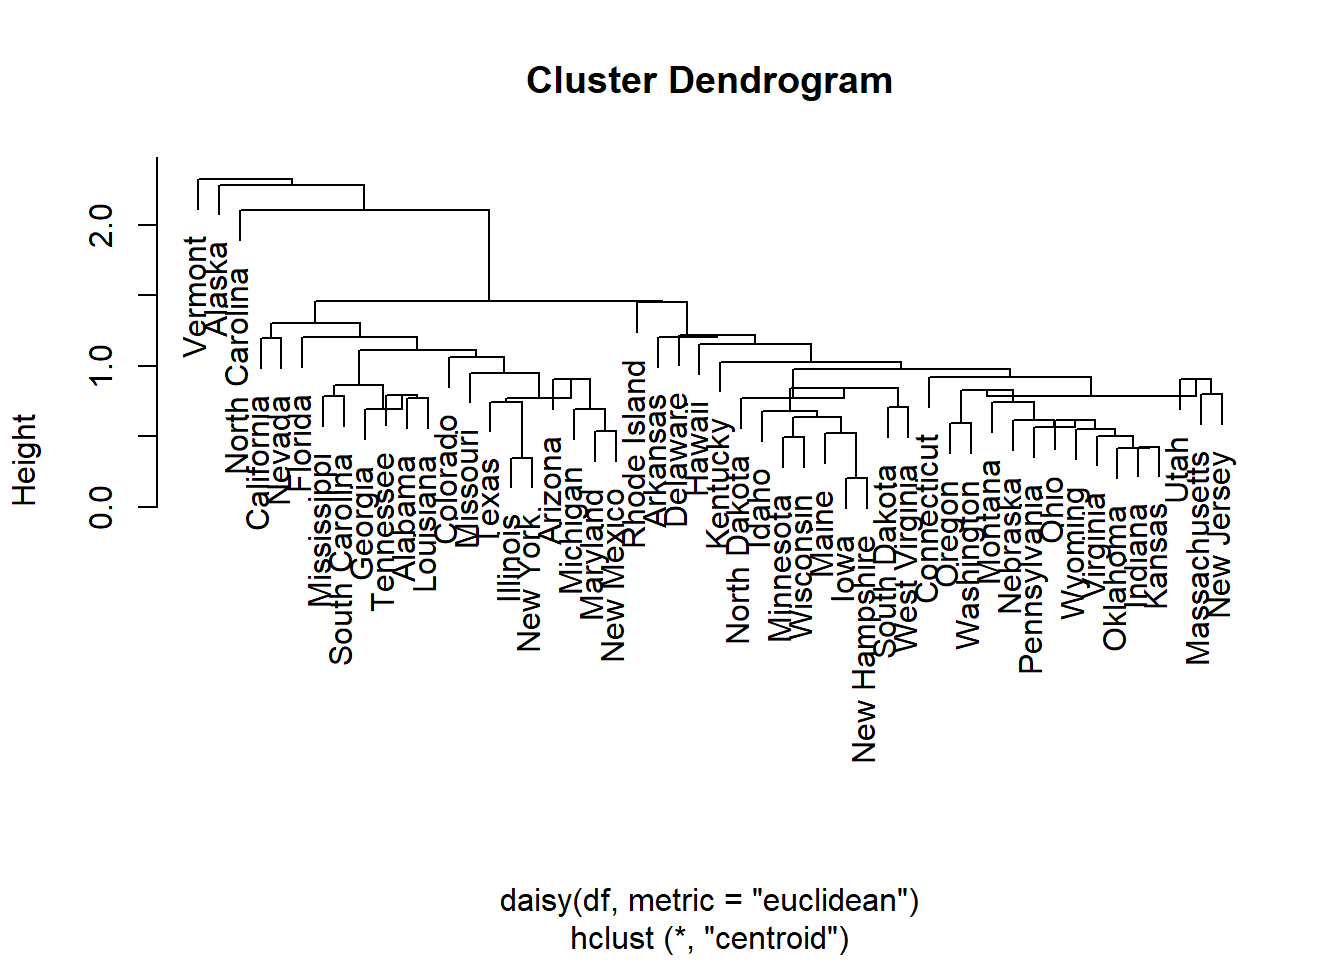
\includegraphics{Unsupervised-Learning_files/figure-latex/unnamed-chunk-27-1.pdf}

According to the elbow method, the optimal number of clusters suggested for the K-means algorithm is 3.

\hypertarget{average-silhouette-method-for-k-means-clustering}{%
\subsection{Average silhouette method for k-means clustering}\label{average-silhouette-method-for-k-means-clustering}}

\begin{Shaded}
\begin{Highlighting}[]
\NormalTok{k.max <-}\StringTok{ }\DecValTok{15}
\NormalTok{data.out <-}\StringTok{ }\NormalTok{df}
\NormalTok{sil <-}\StringTok{ }\KeywordTok{rep}\NormalTok{(}\DecValTok{0}\NormalTok{, k.max)}
\CommentTok{# Compute the average silhouette width for}
\CommentTok{# k = 2 to k = 15}
\ControlFlowTok{for}\NormalTok{(i }\ControlFlowTok{in} \DecValTok{2}\OperatorTok{:}\NormalTok{k.max)\{}
\NormalTok{km.res <-}\StringTok{ }\KeywordTok{kmeans}\NormalTok{(df.out, }\DataTypeTok{centers =}\NormalTok{ i, }\DataTypeTok{nstart =} \DecValTok{25}\NormalTok{)}
\NormalTok{ss <-}\StringTok{ }\KeywordTok{silhouette}\NormalTok{(km.res}\OperatorTok{$}\NormalTok{cluster, }\KeywordTok{dist}\NormalTok{(df.out))}
\NormalTok{sil[i] <-}\StringTok{ }\KeywordTok{mean}\NormalTok{(ss[, }\DecValTok{3}\NormalTok{])}
\NormalTok{\}}
\end{Highlighting}
\end{Shaded}

\begin{Shaded}
\begin{Highlighting}[]
\CommentTok{# Plot the average silhouette width}
\KeywordTok{plot}\NormalTok{(}\DecValTok{1}\OperatorTok{:}\NormalTok{k.max, sil, }\DataTypeTok{type =} \StringTok{"b"}\NormalTok{, }\DataTypeTok{pch =} \DecValTok{19}\NormalTok{,}
\DataTypeTok{frame =} \OtherTok{FALSE}\NormalTok{, }\DataTypeTok{xlab =} \StringTok{"Number of clusters k"}\NormalTok{)}
\KeywordTok{abline}\NormalTok{(}\DataTypeTok{v =} \KeywordTok{which.max}\NormalTok{(sil), }\DataTypeTok{lty =} \DecValTok{2}\NormalTok{)}
\end{Highlighting}
\end{Shaded}

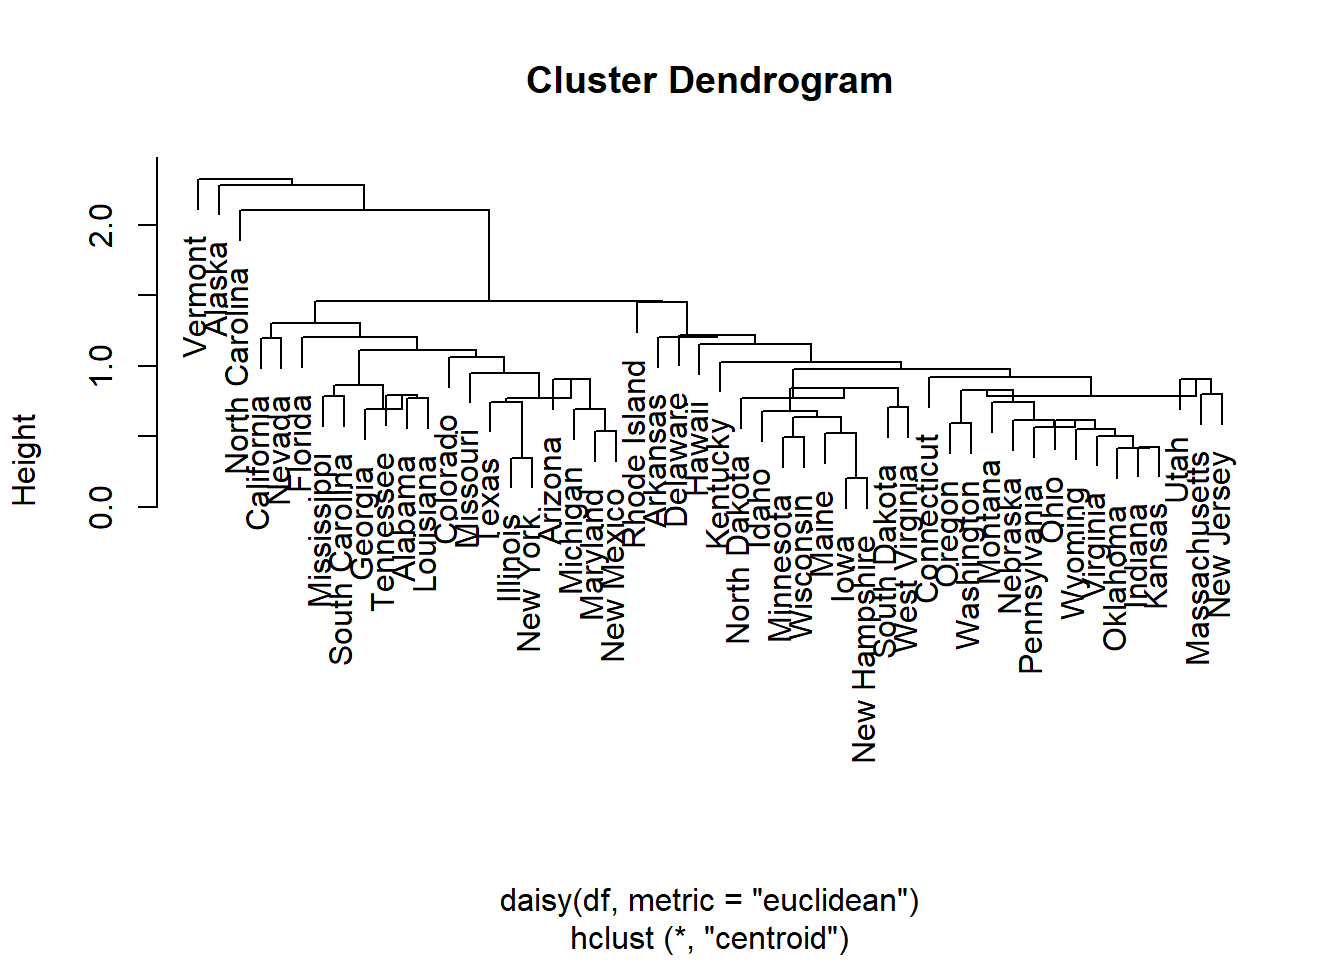
\includegraphics{Unsupervised-Learning_files/figure-latex/unnamed-chunk-29-1.pdf}

According to the silhouette method the optimal number of clusters suggested for the Kmeans algorithm is 2.

\hypertarget{average-silhouette-method-for-pam-clustering}{%
\subsection{Average silhouette method for PAM clustering}\label{average-silhouette-method-for-pam-clustering}}

\begin{Shaded}
\begin{Highlighting}[]
\CommentTok{#clusplot(pam.out, main = "Cluster plot, k = 2", color = TRUE)}
\KeywordTok{plot}\NormalTok{(pam.out)}
\end{Highlighting}
\end{Shaded}

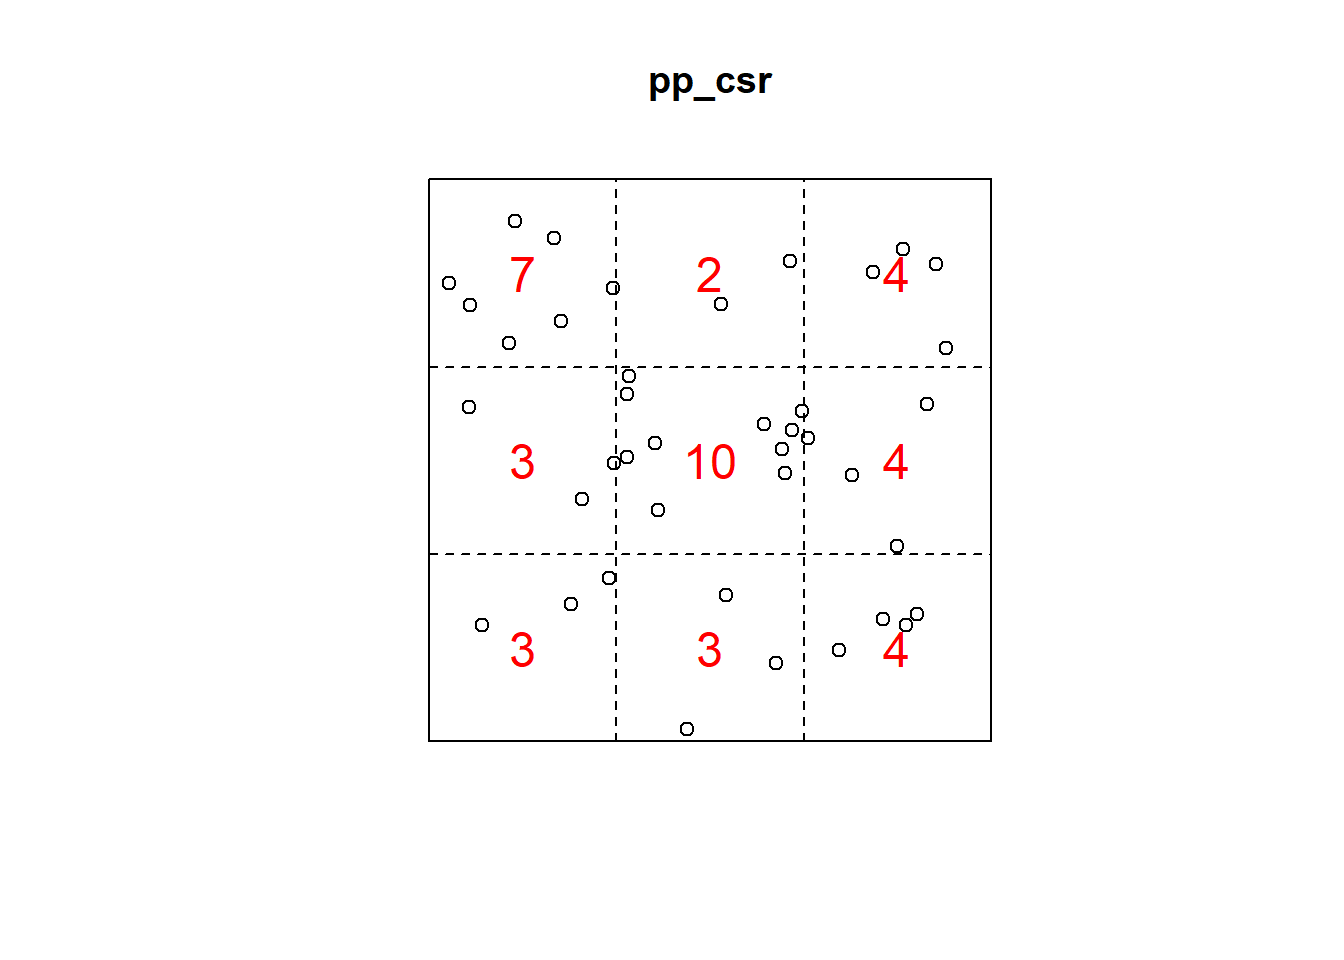
\includegraphics{Unsupervised-Learning_files/figure-latex/unnamed-chunk-30-1.pdf} 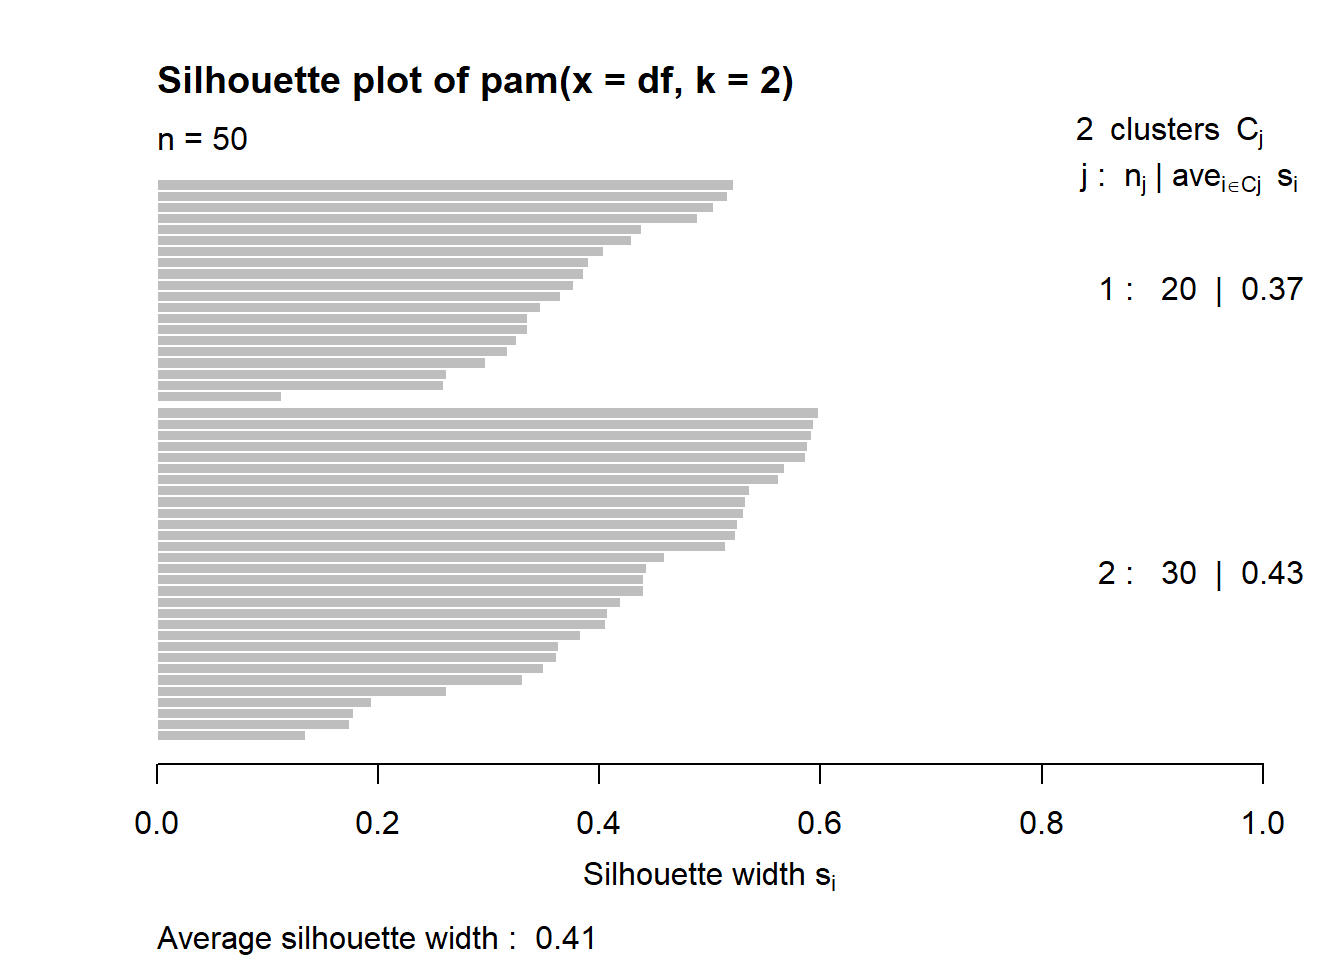
\includegraphics{Unsupervised-Learning_files/figure-latex/unnamed-chunk-30-2.pdf}

These two components explain 86.75\% of the point variability.

This table shows how to use the average silhouette width value:

Range of SC : Interpretation
0.71-1.0 : A strong structure has been found
0.51-0.70 : A reasonable structure has been found
0.26-0.50 : The structure is weak and could be artificial
\textless{} 0.25 : No substantial structure has been found

According to the table, the fit is weak.

\hypertarget{average-silhouette-method-for-hierarchical-clustering}{%
\subsection{Average silhouette method for hierarchical clustering}\label{average-silhouette-method-for-hierarchical-clustering}}

\begin{Shaded}
\begin{Highlighting}[]
\KeywordTok{plot}\NormalTok{(}\KeywordTok{silhouette}\NormalTok{(}\KeywordTok{cutree}\NormalTok{(hc,}\DecValTok{2}\NormalTok{),dist.out))}
\end{Highlighting}
\end{Shaded}

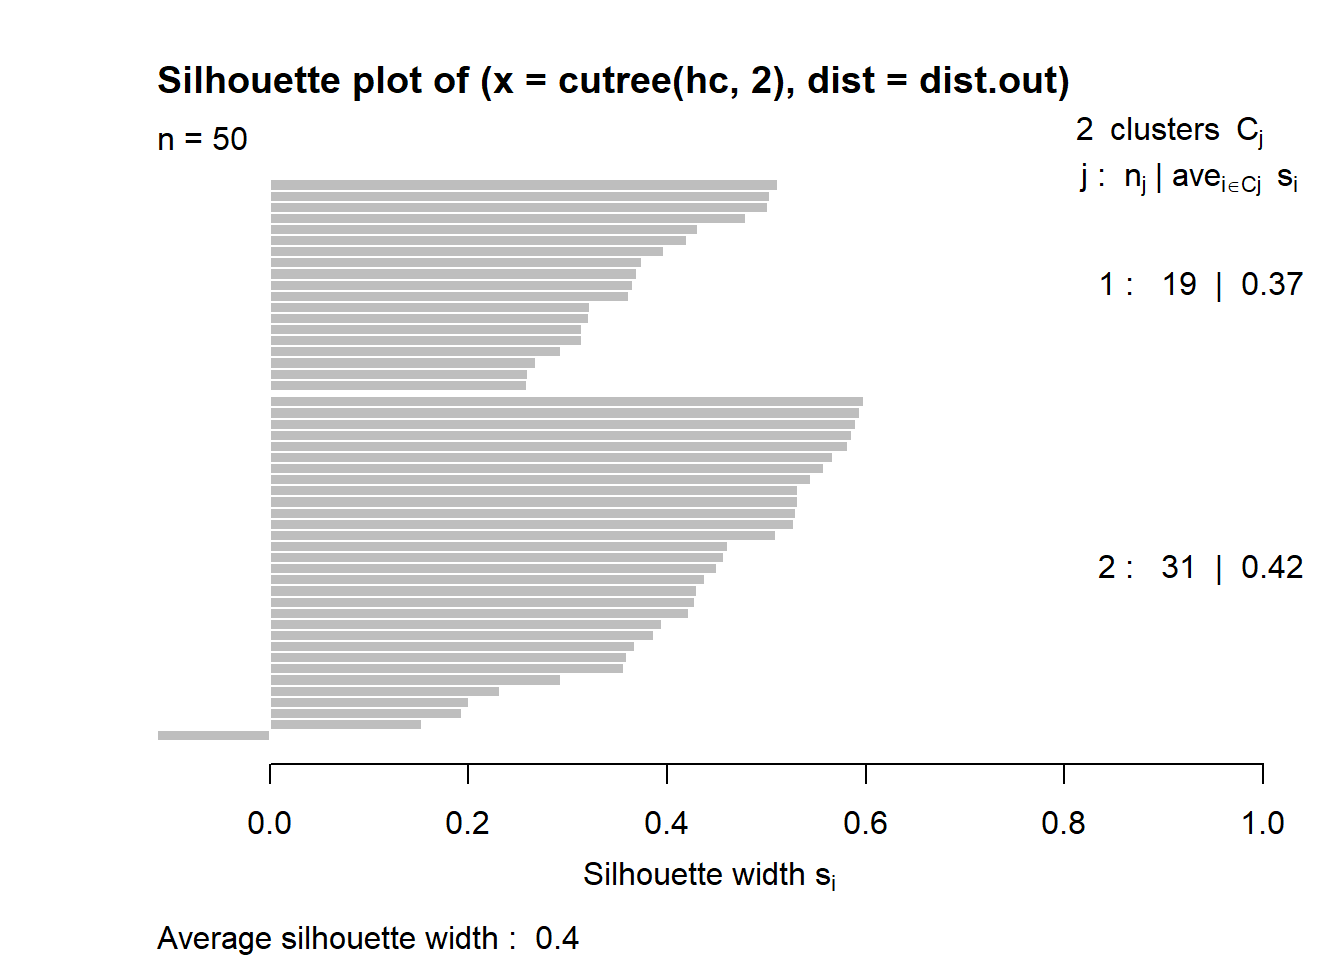
\includegraphics{Unsupervised-Learning_files/figure-latex/unnamed-chunk-31-1.pdf}

Average silhouette width : 0.4

This table shows how to use the average silhouette width value:

Range of SC: Interpretation
0.71-1.0 : A strong structure has been found
0.51-0.70 : A reasonable structure has been found
0.26-0.50 : The structure is weak and could be artificial
\textless{} 0.25 : No substantial structure has been found

The result for hierarchical clustering is similar to that of PAM. The conclusion we can make is that fit is weak.

\hypertarget{gap-statistic-for-k-means-clustering}{%
\subsection{Gap Statistic for K means clustering}\label{gap-statistic-for-k-means-clustering}}

\begin{Shaded}
\begin{Highlighting}[]
\CommentTok{# Compute gap statistic}
\NormalTok{gap_stat <-}\StringTok{ }\KeywordTok{clusGap}\NormalTok{(df, }\DataTypeTok{FUN =}\NormalTok{ kmeans, }\DataTypeTok{nstart =} \DecValTok{25}\NormalTok{, }\DataTypeTok{K.max =} \DecValTok{10}\NormalTok{, }\DataTypeTok{B =} \DecValTok{50}\NormalTok{)}
\CommentTok{# Print the result}
\KeywordTok{plot}\NormalTok{(gap_stat, }\DataTypeTok{frame =} \OtherTok{FALSE}\NormalTok{, }\DataTypeTok{xlab =} \StringTok{"Number of clusters k"}\NormalTok{)}
\KeywordTok{abline}\NormalTok{(}\DataTypeTok{v =} \DecValTok{4}\NormalTok{, }\DataTypeTok{lty =} \DecValTok{2}\NormalTok{)}
\end{Highlighting}
\end{Shaded}

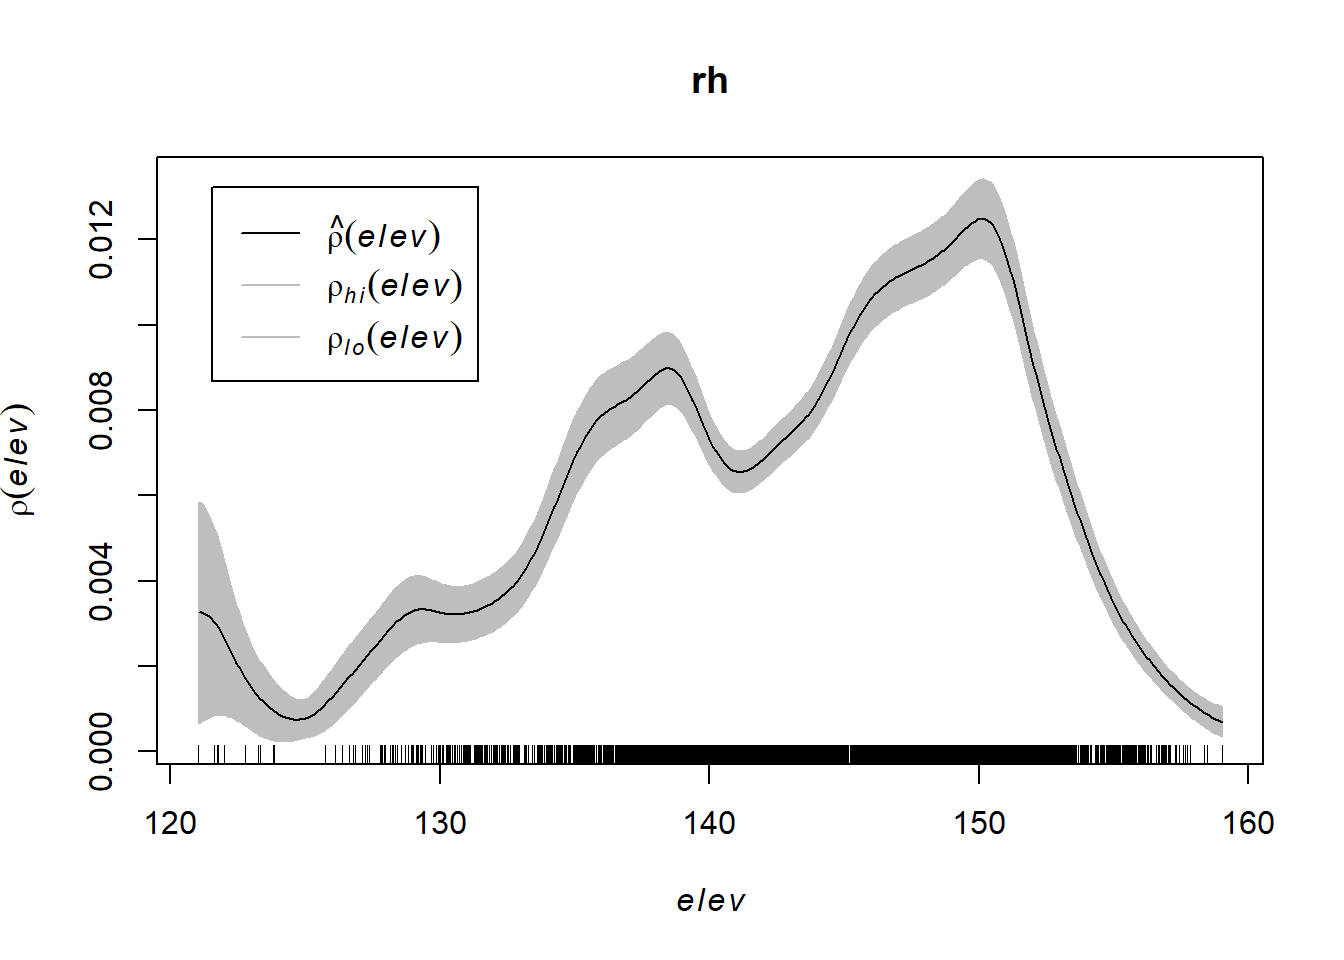
\includegraphics{Unsupervised-Learning_files/figure-latex/unnamed-chunk-32-1.pdf}

According to the Gap Statistic the 'optimal number of clusters chosen for the Kmeans algorithm is 4!

Using the NbClust package which uses a vote to chose the number of clusters.
The following example determine the number of clusters using all statistics:

\begin{Shaded}
\begin{Highlighting}[]
\NormalTok{res.nb <-}\StringTok{ }\KeywordTok{NbClust}\NormalTok{(df, }\DataTypeTok{distance =} \StringTok{"euclidean"}\NormalTok{,}\DataTypeTok{min.nc =} \DecValTok{2}\NormalTok{, max.nc}
\NormalTok{=}\StringTok{ }\DecValTok{10}\NormalTok{, }\DataTypeTok{method =} \StringTok{"complete"}\NormalTok{, }\DataTypeTok{index =}\StringTok{"all"}\NormalTok{)}
\end{Highlighting}
\end{Shaded}

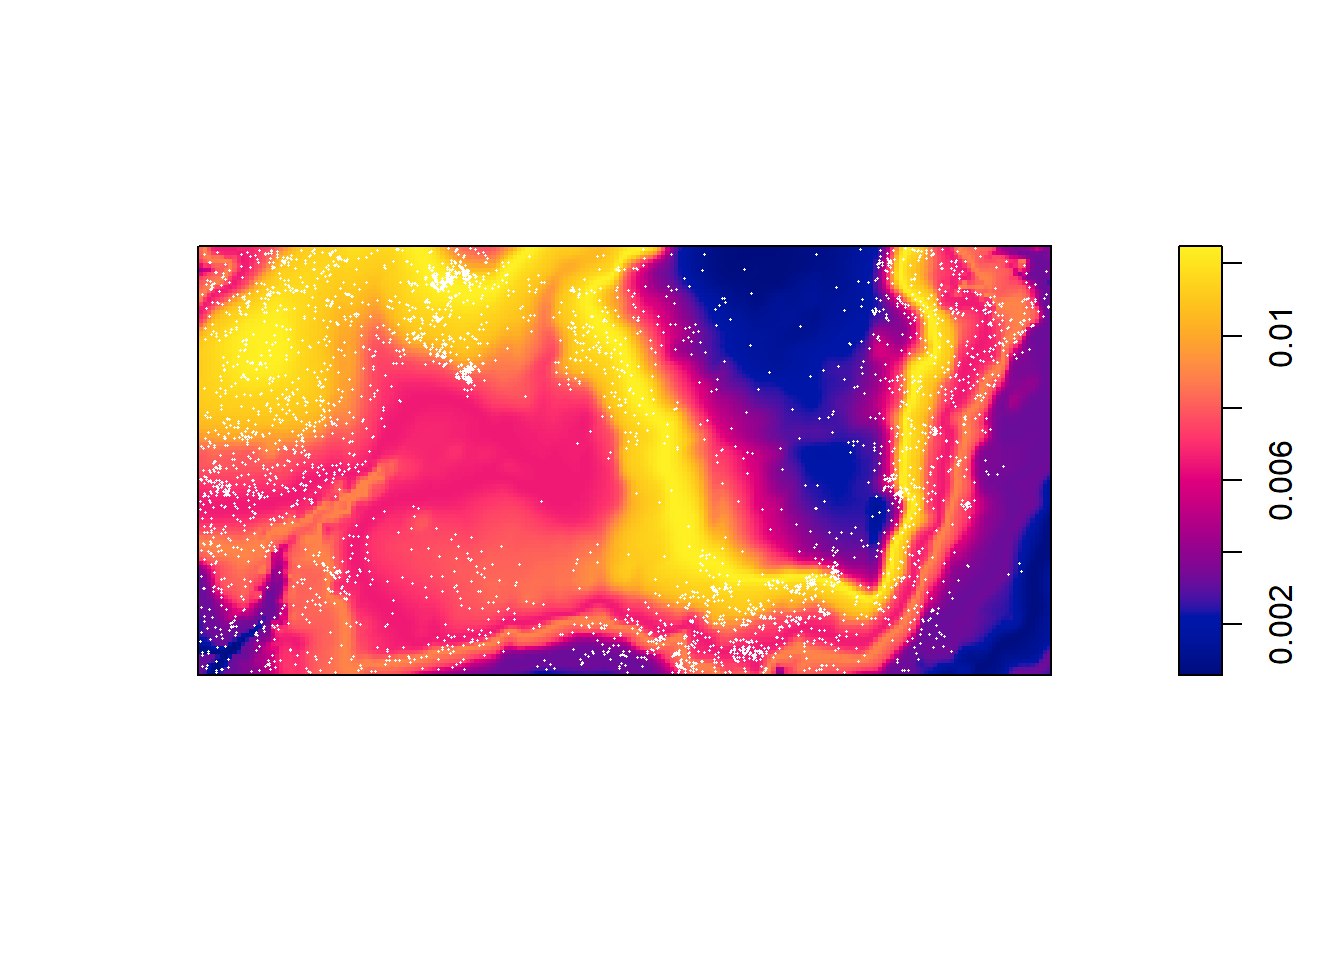
\includegraphics{Unsupervised-Learning_files/figure-latex/unnamed-chunk-33-1.pdf}

\begin{verbatim}
## *** : The Hubert index is a graphical method of determining the number of clusters.
##                 In the plot of Hubert index, we seek a significant knee that corresponds to a 
##                 significant increase of the value of the measure i.e the significant peak in Hubert
##                 index second differences plot. 
## 
\end{verbatim}

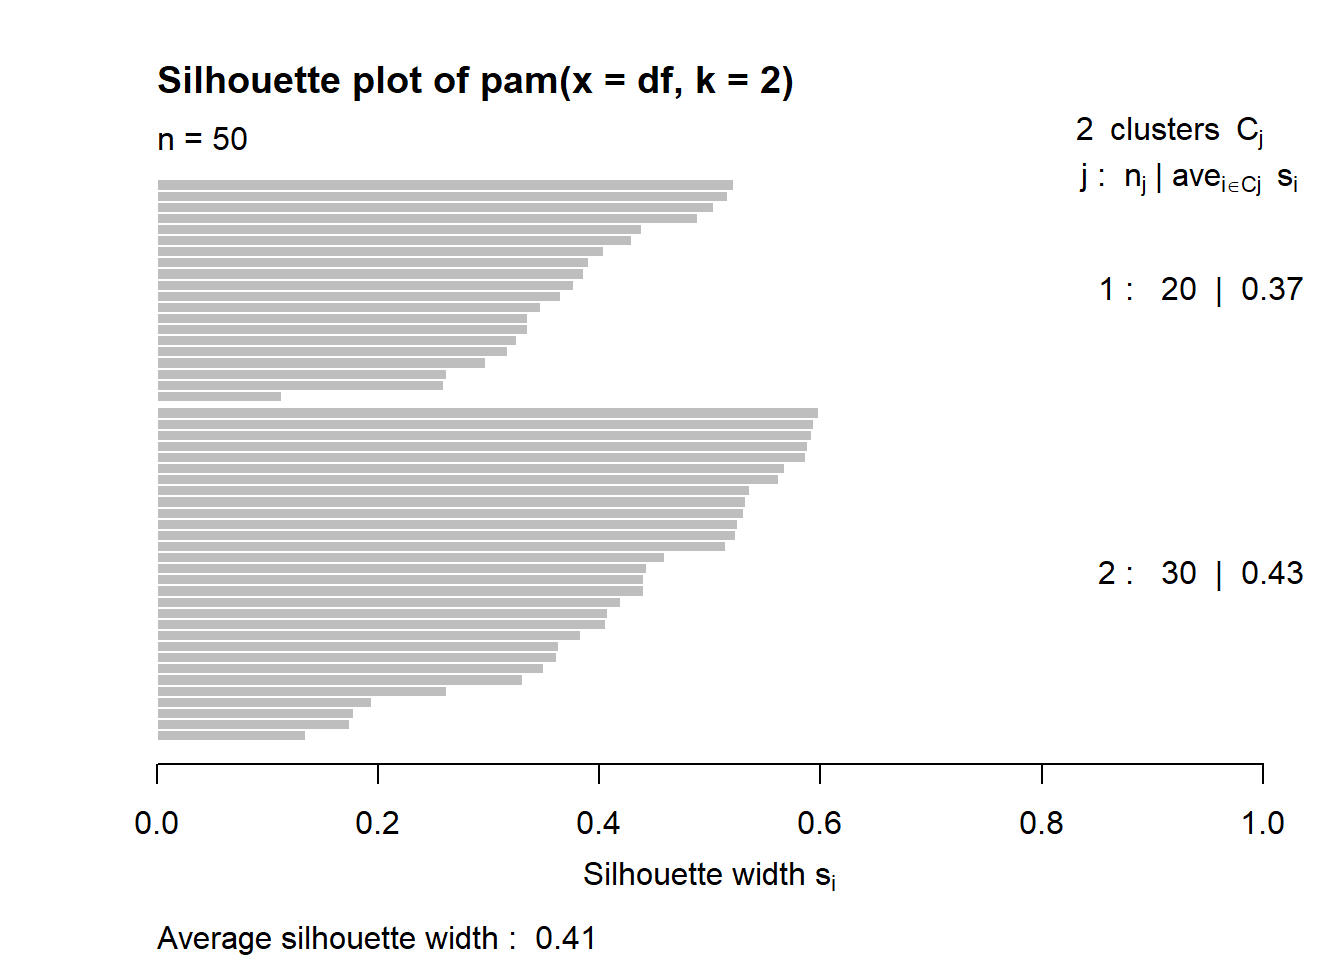
\includegraphics{Unsupervised-Learning_files/figure-latex/unnamed-chunk-33-2.pdf}

\begin{verbatim}
## *** : The D index is a graphical method of determining the number of clusters. 
##                 In the plot of D index, we seek a significant knee (the significant peak in Dindex
##                 second differences plot) that corresponds to a significant increase of the value of
##                 the measure. 
##  
## ******************************************************************* 
## * Among all indices:                                                
## * 9 proposed 2 as the best number of clusters 
## * 4 proposed 3 as the best number of clusters 
## * 6 proposed 4 as the best number of clusters 
## * 2 proposed 5 as the best number of clusters 
## * 1 proposed 8 as the best number of clusters 
## * 1 proposed 10 as the best number of clusters 
## 
##                    ***** Conclusion *****                            
##  
## * According to the majority rule, the best number of clusters is  2 
##  
##  
## *******************************************************************
\end{verbatim}

When all statistics in the NbClust package are allowed to vote, the majority (in this case 9 out of 23) propose
that the `optimal' number of clusters should be 2.

\hypertarget{clustering-with-clara}{%
\section{Clustering with CLARA}\label{clustering-with-clara}}

R function for computing CLARA is found in the in cluster package.

\begin{Shaded}
\begin{Highlighting}[]
\NormalTok{clarax <-}\StringTok{ }\KeywordTok{clara}\NormalTok{(df, }\DecValTok{2}\NormalTok{, }\DataTypeTok{samples=}\DecValTok{10}\NormalTok{)}
\CommentTok{# Silhouette plot}
\KeywordTok{plot}\NormalTok{(}\KeywordTok{silhouette}\NormalTok{(clarax), }\DataTypeTok{col =} \DecValTok{2}\OperatorTok{:}\DecValTok{3}\NormalTok{, }\DataTypeTok{main =} \StringTok{"Silhouette plot"}\NormalTok{)}
\end{Highlighting}
\end{Shaded}

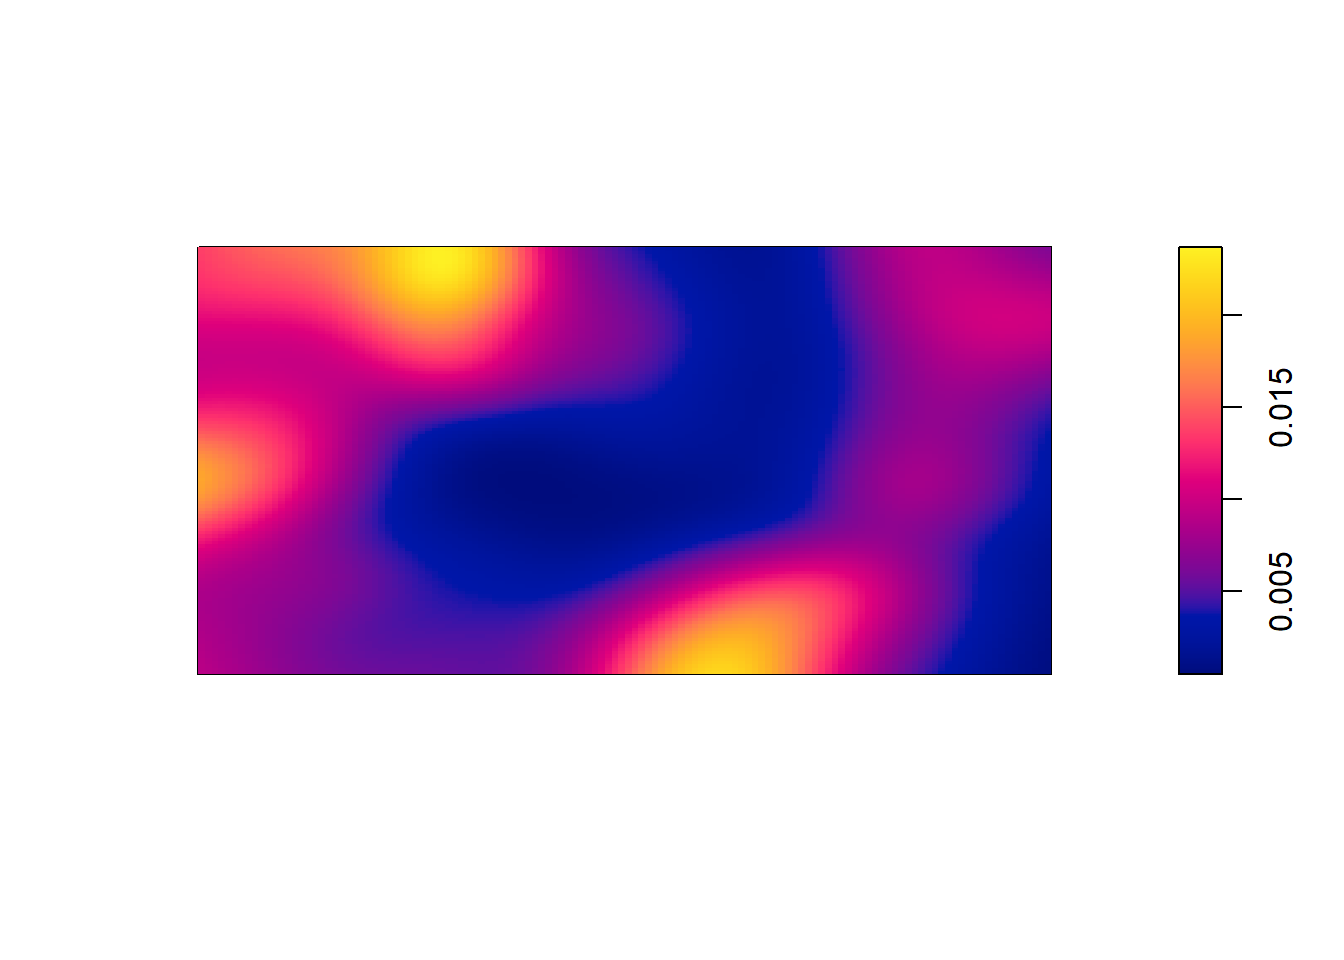
\includegraphics{Unsupervised-Learning_files/figure-latex/unnamed-chunk-34-1.pdf}

The overall average silhouette width is 0.42 meaning that the fit is weak (see table above showing range for Si and corresponding interpretation.

\hypertarget{clustering-with-dbscan}{%
\section{Clustering with DBSCAN}\label{clustering-with-dbscan}}

To illustrate the application of DBSCAN we will use a very simple artificial data set of four slightly overlapping
Gaussians in two-dimensional space with 100 points each. We set the random number generator to make
the results reproducible and create the data set as shown below. The function dbscan() is found in the fpc
package.

\begin{Shaded}
\begin{Highlighting}[]
\KeywordTok{set.seed}\NormalTok{(}\DecValTok{2}\NormalTok{)}
\NormalTok{n <-}\StringTok{ }\DecValTok{400}
\NormalTok{x <-}\StringTok{ }\KeywordTok{cbind}\NormalTok{(}
\DataTypeTok{x =} \KeywordTok{runif}\NormalTok{(}\DecValTok{4}\NormalTok{, }\DecValTok{0}\NormalTok{, }\DecValTok{1}\NormalTok{) }\OperatorTok{+}\StringTok{ }\KeywordTok{rnorm}\NormalTok{(n, }\DataTypeTok{sd =} \FloatTok{0.1}\NormalTok{),}
\DataTypeTok{y =} \KeywordTok{runif}\NormalTok{(}\DecValTok{4}\NormalTok{, }\DecValTok{0}\NormalTok{, }\DecValTok{1}\NormalTok{) }\OperatorTok{+}\StringTok{ }\KeywordTok{rnorm}\NormalTok{(n, }\DataTypeTok{sd =} \FloatTok{0.1}\NormalTok{)}
\NormalTok{)}
\NormalTok{true_clusters <-}\StringTok{ }\KeywordTok{rep}\NormalTok{(}\DecValTok{1}\OperatorTok{:}\DecValTok{4}\NormalTok{, }\DataTypeTok{time =} \DecValTok{100}\NormalTok{)}
\KeywordTok{plot}\NormalTok{(x, }\DataTypeTok{col =}\NormalTok{ true_clusters, }\DataTypeTok{pch =}\NormalTok{ true_clusters)}
\end{Highlighting}
\end{Shaded}

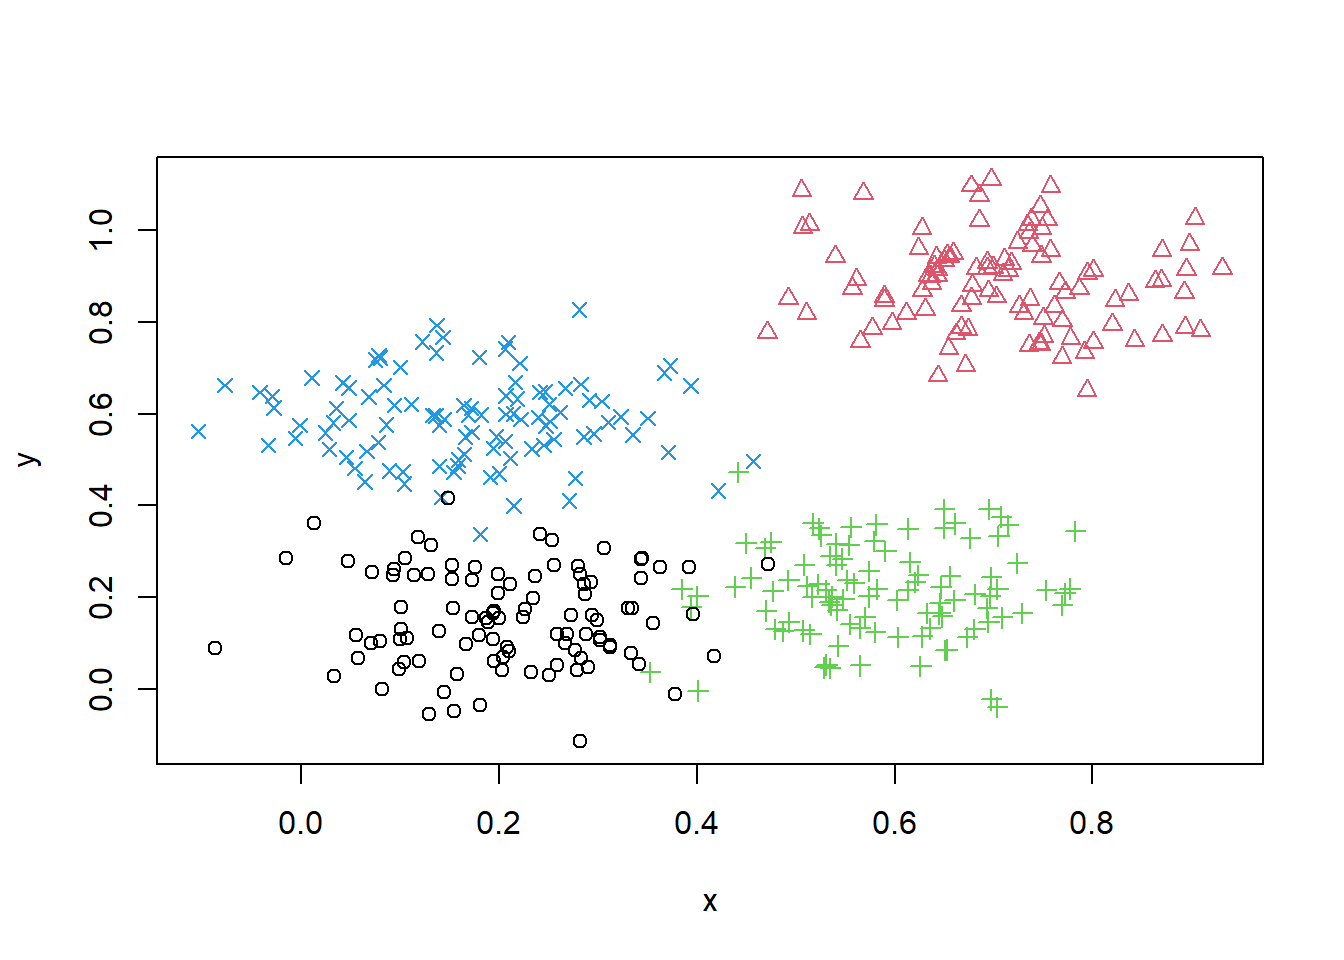
\includegraphics{Unsupervised-Learning_files/figure-latex/unnamed-chunk-35-1.pdf}

\begin{Shaded}
\begin{Highlighting}[]
\CommentTok{# To apply DBSCAN, we need to decide on the neighborhood radius eps}
\CommentTok{# and the density threshold minPts.}
\CommentTok{# The rule of thumb for minPts is to use at least the number of}
\CommentTok{# dimensions of the data set plus one. In our case, this is 3.}
\NormalTok{db <-}\StringTok{ }\NormalTok{fpc}\OperatorTok{::}\KeywordTok{dbscan}\NormalTok{(x, }\DataTypeTok{eps =} \FloatTok{.05}\NormalTok{, }\DataTypeTok{MinPts =}\DecValTok{3}\NormalTok{ )}
\CommentTok{# Plot DBSCAN results}
\KeywordTok{plot}\NormalTok{(db, x, }\DataTypeTok{main =} \StringTok{"DBSCAN"}\NormalTok{, }\DataTypeTok{frame =} \OtherTok{FALSE}\NormalTok{)}
\end{Highlighting}
\end{Shaded}

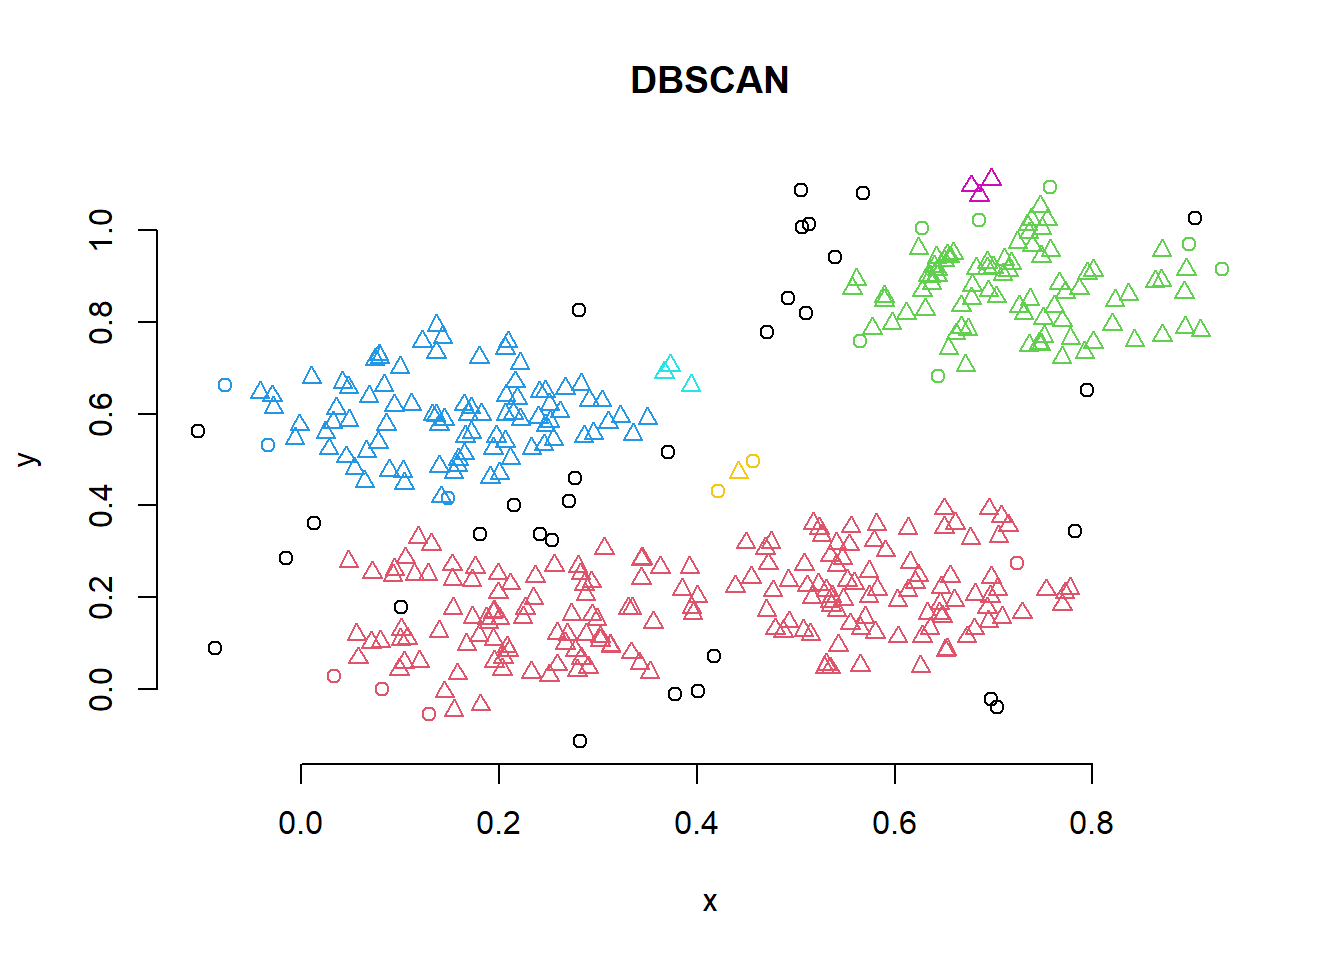
\includegraphics{Unsupervised-Learning_files/figure-latex/unnamed-chunk-36-1.pdf}

DBSCAN has found three clusters in the data.

\hypertarget{clustering-using-mixture-models}{%
\section{Clustering using mixture models}\label{clustering-using-mixture-models}}

For this you need the function Mclust() in the mclust package. There are 14 model options available in
the R package mclust. In one dimension though these collapse into only two models:E for equal variance and
V for varying variance. In more dimensions, the model identifiers encode geometric characteristics of the
model. For example, EVI denotes a model in which the volume of all clusters are equal(E), the shapes of the
clusters may vary (V), and the orientation is the identity (I). That is, clusters in this model have diagonal
covariances with orientation parallel to the coordinate axes.

\begin{Shaded}
\begin{Highlighting}[]
\KeywordTok{library}\NormalTok{(mclust)}
\KeywordTok{data}\NormalTok{(}\StringTok{"diabetes"}\NormalTok{)}
\CommentTok{# Run the function to see how many clusters}
\CommentTok{# it finds to be optimal, set it to search for}
\CommentTok{# at least 1 model and up 20.}
\NormalTok{d_clust <-}\StringTok{ }\KeywordTok{Mclust}\NormalTok{(diabetes[,}\OperatorTok{-}\DecValTok{1}\NormalTok{])}
\KeywordTok{plot}\NormalTok{(d_clust,diabetes[,}\OperatorTok{-}\DecValTok{1}\NormalTok{],}\DataTypeTok{what=}\StringTok{"BIC"}\NormalTok{)}
\end{Highlighting}
\end{Shaded}

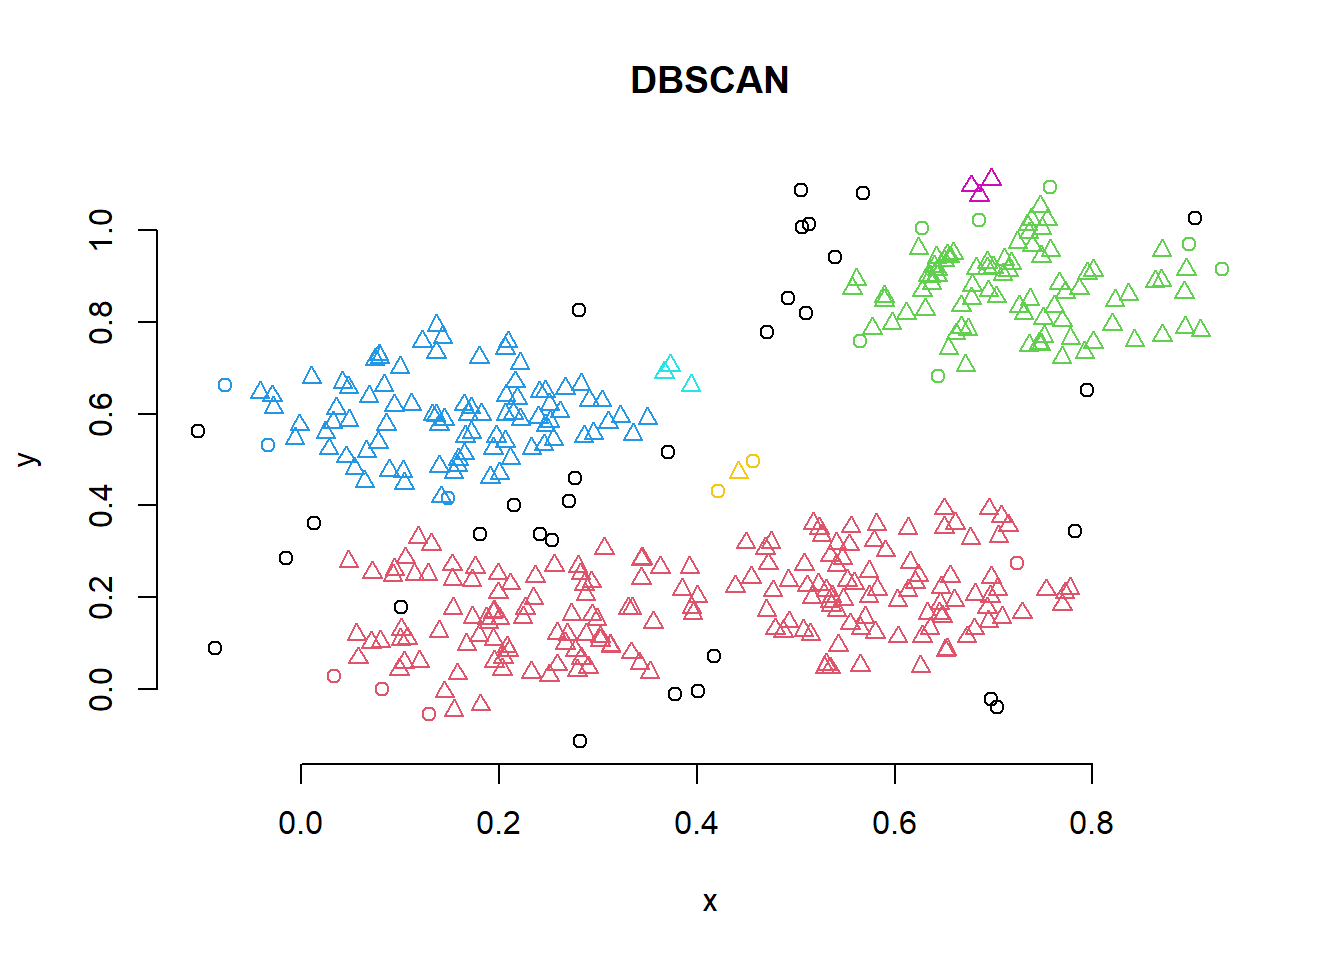
\includegraphics{Unsupervised-Learning_files/figure-latex/unnamed-chunk-37-1.pdf}

The plot shows the results of mclust for the 10 available model parameterizations and up to 9 clusters for the
diabetes dataset. The best model is considered to be the one with the highest BIC among the fitted models.

\begin{Shaded}
\begin{Highlighting}[]
\KeywordTok{coordProj}\NormalTok{(diabetes[,}\OperatorTok{-}\DecValTok{1}\NormalTok{],}\DataTypeTok{dimens =} \KeywordTok{c}\NormalTok{(}\DecValTok{2}\NormalTok{,}\DecValTok{3}\NormalTok{),}\DataTypeTok{what=}\StringTok{"classification"}\NormalTok{,classification}
\NormalTok{=d_clust}\OperatorTok{$}\NormalTok{classification,}\DataTypeTok{parameters =}\NormalTok{ d_clust}\OperatorTok{$}\NormalTok{parameters)}
\end{Highlighting}
\end{Shaded}

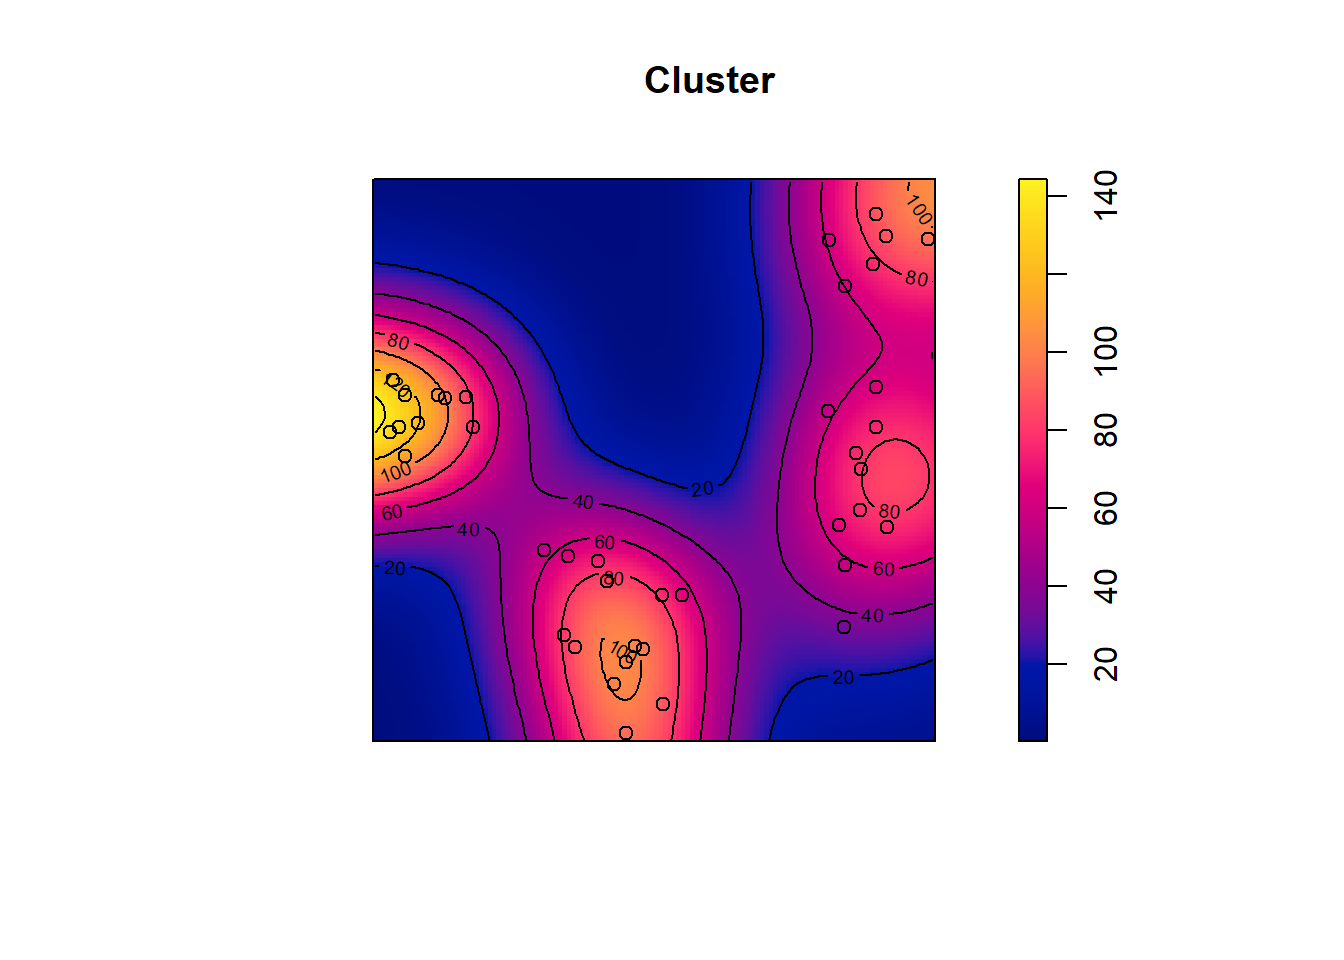
\includegraphics{Unsupervised-Learning_files/figure-latex/unnamed-chunk-38-1.pdf}

This plot shows the projection of the diabetes data with different symbols indicating the classification
corresponding to the best model as determined by mclust. The component means are marked and ellipses
with axes are drawn corresponding to their covariances. In this case there are three components, each with a
different covariance.
For more detailed interpretation see (C.Fraley and A.E. Raftery, Model based Methods of Classification:

Using the mclust Software in Chemometrics. Journal of Statistical Software, Vol. 18, 2007)

\hypertarget{cluster-profiling}{%
\section{Cluster Profiling}\label{cluster-profiling}}

\begin{Shaded}
\begin{Highlighting}[]
\NormalTok{out.complete.euc <-}\StringTok{ }\KeywordTok{hclust}\NormalTok{(}\KeywordTok{daisy}\NormalTok{(df,}\DataTypeTok{metric=}\StringTok{"euclidean"}\NormalTok{),}\DataTypeTok{method=}\StringTok{"complete"}\NormalTok{)}
\KeywordTok{plot}\NormalTok{(out.complete.euc)}
\end{Highlighting}
\end{Shaded}

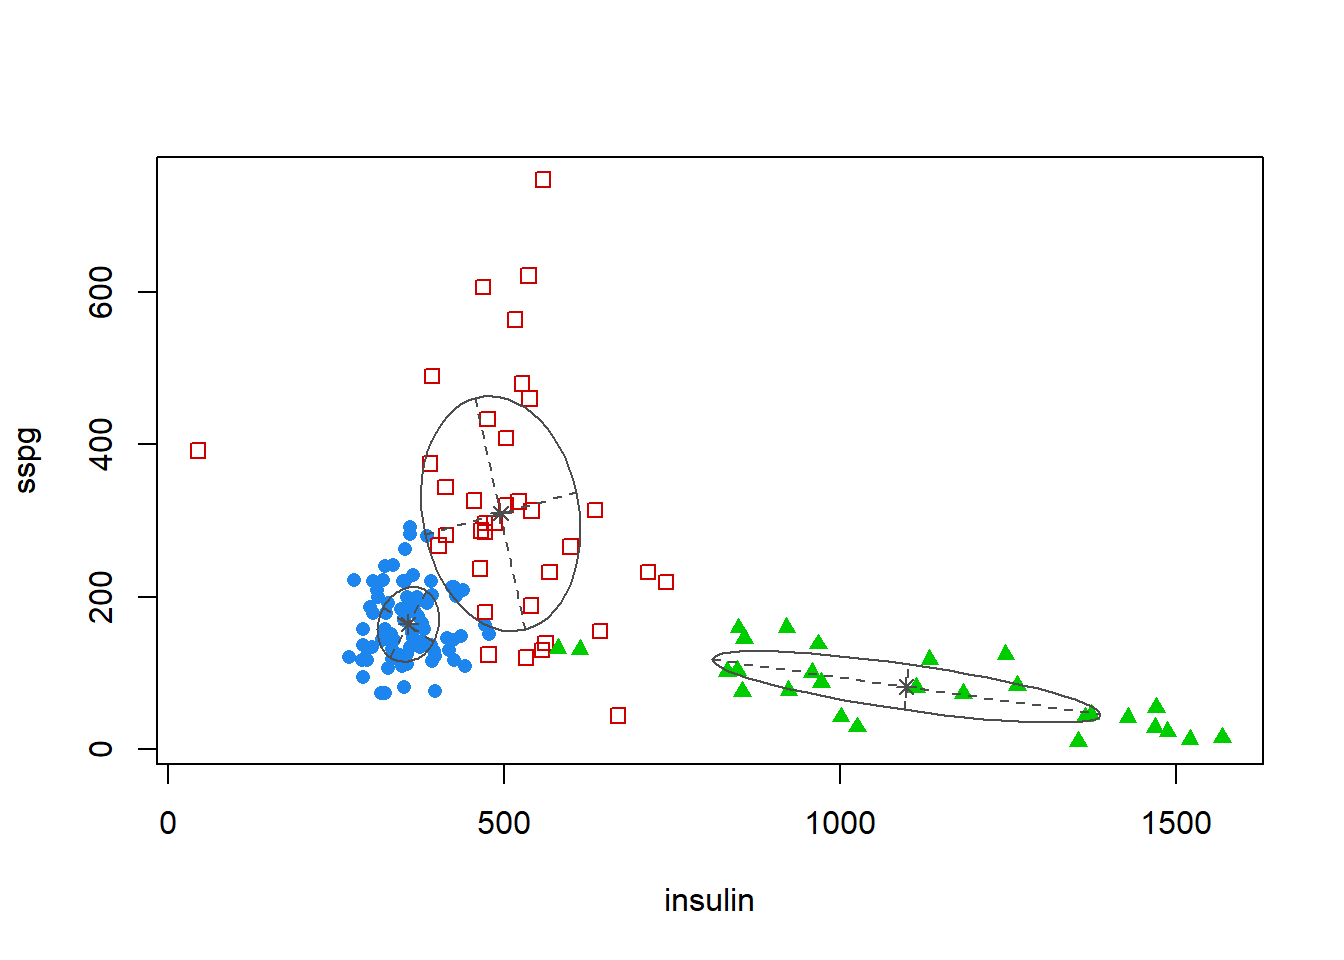
\includegraphics{Unsupervised-Learning_files/figure-latex/unnamed-chunk-39-1.pdf}

\begin{Shaded}
\begin{Highlighting}[]
\NormalTok{out.complete.euc <-}\StringTok{ }\KeywordTok{cutree}\NormalTok{(out.complete.euc, }\DataTypeTok{h=}\FloatTok{3.1}\NormalTok{)}
\NormalTok{clusvec <-}\StringTok{ }\NormalTok{out.complete.euc}
\end{Highlighting}
\end{Shaded}

calculate means

\begin{Shaded}
\begin{Highlighting}[]
\NormalTok{class.means <-}\StringTok{ }\KeywordTok{apply}\NormalTok{(df, }\DecValTok{2}\NormalTok{, }\ControlFlowTok{function}\NormalTok{(x) }\KeywordTok{tapply}\NormalTok{ (x, clusvec, mean))}
\NormalTok{class.means}
\end{Highlighting}
\end{Shaded}

\begin{verbatim}
##       Murder    Assault   UrbanPop        Rape
## 1  1.5803956  0.9662584 -0.7775109  0.04844071
## 2  0.5078625  1.1068225 -1.2117642  2.48420294
## 3  0.7499801  1.1199128  0.9361748  1.21564322
## 4 -0.4400338 -0.4353831  0.3607592 -0.28303852
## 5 -1.0579703 -1.1046626 -1.1219527 -1.02515543
\end{verbatim}

plot means

\begin{Shaded}
\begin{Highlighting}[]
\KeywordTok{plot}\NormalTok{ (}\KeywordTok{c}\NormalTok{(}\DecValTok{1}\NormalTok{,}\KeywordTok{ncol}\NormalTok{(df)),}\KeywordTok{range}\NormalTok{(class.means),}\DataTypeTok{type=}\StringTok{"n"}\NormalTok{,}\DataTypeTok{xlab=}\StringTok{""}\NormalTok{,}\DataTypeTok{ylab=}\StringTok{"Average proportion of protein intake"}\NormalTok{,}\DataTypeTok{xaxt=}\StringTok{"n"}\NormalTok{)}
\KeywordTok{axis}\NormalTok{ (}\DataTypeTok{side=}\DecValTok{1}\NormalTok{, }\DecValTok{1}\OperatorTok{:}\KeywordTok{ncol}\NormalTok{(df), }\KeywordTok{colnames}\NormalTok{(df), }\DataTypeTok{las=}\DecValTok{2}\NormalTok{)}
\CommentTok{#ensure you list enough colours for the number of clusters}
\NormalTok{colvec <-}\StringTok{ }\KeywordTok{c}\NormalTok{(}\StringTok{"green"}\NormalTok{,}\StringTok{"gold"}\NormalTok{,}\StringTok{"blue"}\NormalTok{,}\StringTok{"red"}\NormalTok{,}\StringTok{"black"}\NormalTok{)}
\ControlFlowTok{for}\NormalTok{ (i }\ControlFlowTok{in} \DecValTok{1}\OperatorTok{:}\KeywordTok{nrow}\NormalTok{(class.means))}
  \KeywordTok{lines}\NormalTok{ (}\DecValTok{1}\OperatorTok{:}\KeywordTok{ncol}\NormalTok{(df),class.means[i,],}\DataTypeTok{col=}\NormalTok{colvec[i])}
\end{Highlighting}
\end{Shaded}

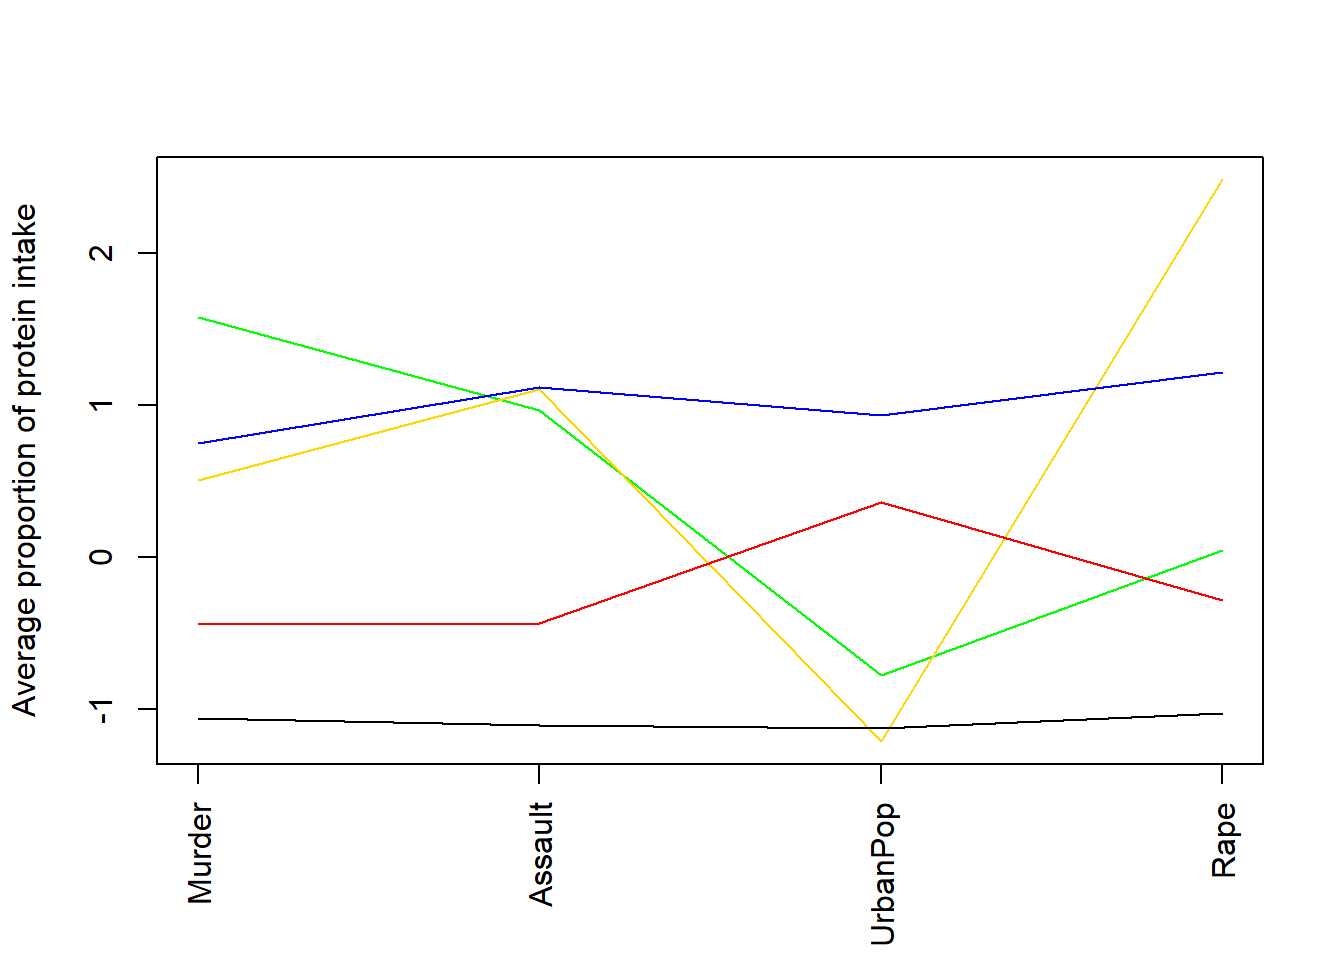
\includegraphics{Unsupervised-Learning_files/figure-latex/unnamed-chunk-41-1.pdf}

\hypertarget{self-organising-maps}{%
\chapter{Self Organising Maps}\label{self-organising-maps}}

For this section, please update your browser on the 20th of October Tuesday.

  \bibliography{book.bib,packages.bib}

\end{document}
